% Template adapted from https://github.com/jgm/pandoc-templates/blob/master/default.latex
% To be used with XeLaTex in memoiR
%%%%%%%%%%%%%%%%%%%%%%%%%%%%%%%%%%%%%%%%%%%%%%%%%%%%%%%%%%%%%%%%%%%%%%%%%%%%%%%%%%%%%%%%%

% Options for packages loaded elsewhere
\PassOptionsToPackage{unicode=true}{hyperref}
\PassOptionsToPackage{hyphens}{url}
\PassOptionsToPackage{dvipsnames,svgnames*,x11names*}{xcolor}
% Right to left support


\documentclass[
  10pt,
  italian,
  a4paper,
  extrafontsizes,onecolumn,openright
  ]{memoir}

% Double (or whatever) spacing

% Math
\usepackage{amssymb, amsmath}
% mathspec: arbitrary math fonts
\usepackage{unicode-math}
\defaultfontfeatures{Scale=MatchLowercase}
\defaultfontfeatures[\rmfamily]{Ligatures=TeX,Scale=1}

% Fonts
\usepackage{lmodern}
\usepackage{fontspec}

% Main font
% Specific sanserif font
% Specific monotype font
\setmonofont[Scale=0.75]{Operator Mono SSm Lig Book}
% Specific math font
% Chinese, Japanese, Corean fonts

% Use upquote for straight quotes in verbatim environments
\usepackage{upquote}
% Use microtype
\usepackage[]{microtype}
\UseMicrotypeSet[protrusion]{basicmath} % disable protrusion for tt fonts

% Verbatim in note

% Color links
\usepackage{xcolor}

% Strikeout

% Necessary for code chunks
\usepackage{color}
\usepackage{fancyvrb}
\newcommand{\VerbBar}{|}
\newcommand{\VERB}{\Verb[commandchars=\\\{\}]}
\DefineVerbatimEnvironment{Highlighting}{Verbatim}{commandchars=\\\{\}}
% Add ',fontsize=\small' for more characters per line
\usepackage{framed}
\definecolor{shadecolor}{RGB}{248,248,248}
\newenvironment{Shaded}{\begin{snugshade}}{\end{snugshade}}
\newcommand{\AlertTok}[1]{\textcolor[rgb]{0.94,0.16,0.16}{#1}}
\newcommand{\AnnotationTok}[1]{\textcolor[rgb]{0.56,0.35,0.01}{\textbf{\textit{#1}}}}
\newcommand{\AttributeTok}[1]{\textcolor[rgb]{0.77,0.63,0.00}{#1}}
\newcommand{\BaseNTok}[1]{\textcolor[rgb]{0.00,0.00,0.81}{#1}}
\newcommand{\BuiltInTok}[1]{#1}
\newcommand{\CharTok}[1]{\textcolor[rgb]{0.31,0.60,0.02}{#1}}
\newcommand{\CommentTok}[1]{\textcolor[rgb]{0.56,0.35,0.01}{\textit{#1}}}
\newcommand{\CommentVarTok}[1]{\textcolor[rgb]{0.56,0.35,0.01}{\textbf{\textit{#1}}}}
\newcommand{\ConstantTok}[1]{\textcolor[rgb]{0.00,0.00,0.00}{#1}}
\newcommand{\ControlFlowTok}[1]{\textcolor[rgb]{0.13,0.29,0.53}{\textbf{#1}}}
\newcommand{\DataTypeTok}[1]{\textcolor[rgb]{0.13,0.29,0.53}{#1}}
\newcommand{\DecValTok}[1]{\textcolor[rgb]{0.00,0.00,0.81}{#1}}
\newcommand{\DocumentationTok}[1]{\textcolor[rgb]{0.56,0.35,0.01}{\textbf{\textit{#1}}}}
\newcommand{\ErrorTok}[1]{\textcolor[rgb]{0.64,0.00,0.00}{\textbf{#1}}}
\newcommand{\ExtensionTok}[1]{#1}
\newcommand{\FloatTok}[1]{\textcolor[rgb]{0.00,0.00,0.81}{#1}}
\newcommand{\FunctionTok}[1]{\textcolor[rgb]{0.00,0.00,0.00}{#1}}
\newcommand{\ImportTok}[1]{#1}
\newcommand{\InformationTok}[1]{\textcolor[rgb]{0.56,0.35,0.01}{\textbf{\textit{#1}}}}
\newcommand{\KeywordTok}[1]{\textcolor[rgb]{0.13,0.29,0.53}{\textbf{#1}}}
\newcommand{\NormalTok}[1]{#1}
\newcommand{\OperatorTok}[1]{\textcolor[rgb]{0.81,0.36,0.00}{\textbf{#1}}}
\newcommand{\OtherTok}[1]{\textcolor[rgb]{0.56,0.35,0.01}{#1}}
\newcommand{\PreprocessorTok}[1]{\textcolor[rgb]{0.56,0.35,0.01}{\textit{#1}}}
\newcommand{\RegionMarkerTok}[1]{#1}
\newcommand{\SpecialCharTok}[1]{\textcolor[rgb]{0.00,0.00,0.00}{#1}}
\newcommand{\SpecialStringTok}[1]{\textcolor[rgb]{0.31,0.60,0.02}{#1}}
\newcommand{\StringTok}[1]{\textcolor[rgb]{0.31,0.60,0.02}{#1}}
\newcommand{\VariableTok}[1]{\textcolor[rgb]{0.00,0.00,0.00}{#1}}
\newcommand{\VerbatimStringTok}[1]{\textcolor[rgb]{0.31,0.60,0.02}{#1}}
\newcommand{\WarningTok}[1]{\textcolor[rgb]{0.56,0.35,0.01}{\textbf{\textit{#1}}}}

% Listings package

% Tables
\usepackage{longtable,booktabs,tabu}
% Fix footnotes in tables (requires footnote package)
\IfFileExists{footnote.sty}{\usepackage{footnote}\makesavenoteenv{longtable}}{}

% Graphics
\usepackage{graphicx,grffile}
\graphicspath{{images/}}
\makeatletter
\def\maxwidth{\ifdim\Gin@nat@width>\linewidth\linewidth\else\Gin@nat@width\fi}
\def\maxheight{\ifdim\Gin@nat@height>\textheight\textheight\else\Gin@nat@height\fi}
\makeatother
% Scale images if necessary, so that they will not overflow the page
% margins by default, and it is still possible to overwrite the defaults
% using explicit options in \includegraphics[width, height, ...]{}
\setkeys{Gin}{width=\maxwidth,height=\maxheight,keepaspectratio}

% Prevent overfull lines
\setlength{\emergencystretch}{3em}  
\providecommand{\tightlist}{%
  \setlength{\itemsep}{0pt}\setlength{\parskip}{0pt}}

% Number sections for memoir (secnumdepth counter is ignored)
\setsecnumdepth{section}

% Set default figure placement to htbp
\makeatletter
\def\fps@figure{htbp}
\makeatother

% Spacing in lists
\usepackage{enumitem}

% Polyglossia
\usepackage{polyglossia}
\setmainlanguage{it}
\setotherlanguage{en-US}

% BibLaTeX
\usepackage[backend=biber,style=authoryear-ibid,isbn=false,backref=true,giveninits=true,uniquename=init,maxcitenames=2,maxbibnames=150,sorting=nyt,sortcites=false,style=apa]{biblatex}
\addbibresource{refs.bib}

% cslreferences environment required by pandoc > 2.7



%%%%%%%%%%%%%%%%%%%%%%%%%%%%%%%%%%%%%%%%%%%%%%%%%%%%%%%%%%
% memoiR format

% Chapter Summary environment 
\usepackage[tikz]{bclogo}
\newenvironment{Summary}
  {\begin{bclogo}[logo=\bctrombone, noborder=true, couleur=lightgray!50]{In breve}\parindent0pt}
  {\end{bclogo}}
% Syntax:
%
%```{block, type='Summary'}
% Deliver message here.
% ```

% scriptsize code 
\let\oldverbatim\verbatim
\def\verbatim{\oldverbatim\scriptsize}
% Applies to code blocks and R code results
% code chunk options size='scriptsize' applies only to R code and results
% if the code chunk sets a different size, \def\verbatim{...} is prioritary for code results 


% Layout
%%%%%%%%%%%%%%%%%%%%%%%%%%%%%%%%%%%%%%%%%%%%%%%%%%%%%%%%%%

% Based on memoir, style companion
\newcommand{\MemoirChapStyle}{daleif1}
\newcommand{\MemoirPageStyle}{Ruled}

% Space between paragraphs
\usepackage{parskip}
  \abnormalparskip{3pt}

% Adjust margin paragraphs vertical position
\usepackage{marginfix}


% Margins
%%%%%%%%%%%%%%%%%%%%%%%%%%%%%%%%%%%%%%%

% allow use of '-',+','/' ans '*' to make simple length computation
\usepackage{calc}

% Full-width figures utilities
\newlength\widthw % full width
\newlength{\rf}
\newcommand*{\definesHSpace}{
  \strictpagecheck % slower but efficient detection of odd/even pages
  \checkoddpage
  \ifoddpage
  \setlength{\rf}{0mm}
  \else
  \setlength{\rf}{\marginparsep+\marginparwidth}
  \fi
}

\makeatletter
% 1" margins for the front matter.
\newcommand*{\SmallMargins}{
  \setlrmarginsandblock{1.5in}{1.5in}{*}
  \setmarginnotes{0.1in}{0.1in}{0.1in}
 \setulmarginsandblock{1.5in}{1in}{*}
  \checkandfixthelayout
  \ch@ngetext
  \clearpage
  \setlength{\widthw}{\textwidth+\marginparsep+\marginparwidth}
  \footnotesatfoot
  \chapterstyle{\MemoirChapStyle}  % Chapter and page styles must be recalled
  \pagestyle{\MemoirPageStyle}
}

% 3" outer margin for the main matter
\newcommand{\LargeMargins}{\SmallMargins}
\makeatother

% Figure captions and footnotes in outer margins


% Main title page with filigrane
%%%%%%%%%%%%%%%%%%%%%%%%%%%%%%%%%%%%%%%%%%%%%%%%%%%%%%%%%%

% Text blocks
\usepackage[absolute,overlay]{textpos}
  \setlength{\TPHorizModule}{1mm}
  \setlength{\TPVertModule}{1mm}

\newcommand{\MainTitlePage}[2]{
  \SmallMargins % Margins
  \pagestyle{empty} % No header/footer
  \textblockorigin{\stockwidth-\paperwidth-\trimedge}{\trimtop} % recto
  \begin{textblock*}{2mm}(\spinemargin/2,\uppermargin/2)
    \rule{1pt}{\paperheight-\uppermargin}
  \end{textblock*}
  \begin{textblock*}{\paperwidth*2/3}(\paperwidth/5, \paperheight/5)
    \flushright
    \begin{Spacing}{3}
      {\fontfamily{qtm}\selectfont\fontsize{45}{45}\selectfont\textsc{\thetitle}}
    \end{Spacing}
  \end{textblock*}
    \begin{textblock*}{\paperwidth*2/3}(\paperwidth/5, \paperheight/2)
    \flushright
    {\fontfamily{qtm}\huge\theauthor}
  \end{textblock*}
    \begin{textblock*}{\paperwidth*2/3}[0, 1](\spinemargin, \uppermargin+\textheight)
    \normalfont\thedate
  \end{textblock*}
  ~\\ % Print a character or the page will not exist
  \newpage
  \textblockorigin{\trimedge}{\trimtop} % verso
  \begin{textblock*}{\textwidth}(\paperwidth-\spinemargin-\textwidth, \uppermargin)
    #1
  \end{textblock*}
  \begin{textblock*}{\textwidth}[0,1](\paperwidth-\spinemargin-\textwidth, \uppermargin+\textheight+\footskip)
    \centering
    
\includegraphics[width=\paperwidth/4]{logo}\\ \bigskip
    #2
  \end{textblock*}
  ~\\ % Print a character or the page will not exist
  \newpage
}

% Clear page and open an even one (\clearpage opens an odd one)
\newcommand{\evenpage}{
  \clearpage
  \strictpagecheck % slower but efficient detection of odd/even pages
  \checkoddpage
  \ifoddpage
    \thispagestyle{empty}
    ~\\ % Print a character or the page will not exist
    \newpage
  \else
    % do nothing
  \fi
}


%% PDF title page to insert
%%%%%%%%%%%%%%%%%%%%%%%%%%%%%%%%%%%%%%%%%%%%%%%%%%%%%%%%%%



%% Bibliography
%%%%%%%%%%%%%%%%%%%%%%%%%%%%%%%%%%%%%%%%%%%%%%%%%%%%%%%%%%

\usepackage[strict,autostyle]{csquotes}
% Repeated citation as author-year-title instead of author-title (modification of footcite:note in verbose-inote.cbx)

%% Table of Contents
%%%%%%%%%%%%%%%%%%%%%%%%%%%%%%%%%%%%%%%%%%%%%%%%%%%%%%%%%%

% fix the typesetting of the part number
\renewcommand\partnumberlinebox[2]{#2\ ---\ }


% Fonts
%%%%%%%%%%%%%%%%%%%%%%%%%%%%%%%%%%%%%%%%%%%%%%%%%%%%%%%%%%


% Hyperref comes last
%%%%%%%%%%%%%%%%%%%%%%%%%%%%%%%%%%%%%%%%%%%%%%%%%%%%%%%%%%

\usepackage{hyperref}
\hypersetup{
  pdftitle={Psicometria},
  pdfauthor={Corrado Caudek},
  colorlinks=true,
  linkcolor=Maroon,
  citecolor=Blue,
  urlcolor=Blue,
  breaklinks=true}

% Don't use monospace font for urls
\urlstyle{same}


% Title, author, date from YAML to LaTeX
%%%%%%%%%%%%%%%%%%%%%%%%%%%%%%%%%%%%%%%%%%%%%%%%%%%%%%%%%%

\title{Psicometria}

\author{Corrado Caudek}

\date{2021-12-04}


% Include headers (preamble.tex) here
%%%%%%%%%%%%%%%%%%%%%%%%%%%%%%%%%%%%%%%%%%%%%%%%%%%%%%%%%%
% Add LaTeX code into the preamble of the document here
\hyphenation{bio-di-ver-si-ty sap-lings}


%%%%%%%%%%%%%%%%%%%%%%%%%%%%%%%%%%%%%%%%%%%%%%%%%%%%%%%%%%%%%%%%%%%%%%%%%
% memoiR dalef3 chapter style 
% https://ctan.crest.fr/tex-archive/info/latex-samples/MemoirChapStyles/MemoirChapStyles.pdf
\usepackage{soul}
\definecolor{nicered}{rgb}{.647,.129,.149}
\makeatletter
\newlength\dlf@normtxtw
\setlength\dlf@normtxtw{\textwidth}
\def\myhelvetfont{\def\sfdefault{mdput}}
\newsavebox{\feline@chapter}
\newcommand\feline@chapter@marker[1][4cm]{%
  \sbox\feline@chapter{%
    \resizebox{!}{#1}{\fboxsep=1pt%
	  \colorbox{nicered}{\color{white}\bfseries\sffamily\thechapter}%
	}}%
  \rotatebox{90}{%
    \resizebox{%
	  \heightof{\usebox{\feline@chapter}}+\depthof{\usebox{\feline@chapter}}}%
	{!}{\scshape\so\@chapapp}}\quad%
  \raisebox{\depthof{\usebox{\feline@chapter}}}{\usebox{\feline@chapter}}%
 }
\newcommand\feline@chm[1][4cm]{%
  \sbox\feline@chapter{\feline@chapter@marker[#1]}%
  \makebox[0pt][l]{% aka \rlap
    \makebox[1cm][r]{\usebox\feline@chapter}%
  }}
\makechapterstyle{daleif1}{
  \renewcommand\chapnamefont{\normalfont\Large\scshape\raggedleft\so}
  \renewcommand\chaptitlefont{\normalfont\huge\bfseries\scshape\color{nicered}}
  \renewcommand\chapternamenum{}
  \renewcommand\printchaptername{}
  \renewcommand\printchapternum{\null\hfill\feline@chm[2.5cm]\par}
  \renewcommand\afterchapternum{\par\vskip\midchapskip}
  \renewcommand\printchaptertitle[1]{\chaptitlefont\raggedleft ##1\par}
}
\makeatother

\DeclareMathOperator{\Var}{Var} % Define variance operator
\DeclareMathOperator{\SD}{SD} % Define sd operator
\DeclareMathOperator{\Cov}{Cov} % Define covariance operator
\DeclareMathOperator{\Corr}{Corr} % Define correlation operator
\DeclareMathOperator{\Me}{Me} % Define mediane operator
\DeclareMathOperator{\Mo}{Mo} % Define mode operator
\DeclareMathOperator{\Bin}{Bin} % Define binomial operator
\DeclareMathOperator{\Bernoulli}{Bernoulli} % Define Bernoulli operator
\DeclareMathOperator{\Poi}{Poi} % Define Poisson operator
\DeclareMathOperator{\Uniform}{Uniform} % Define Uniform operator
\DeclareMathOperator{\Cauchy}{Cauchy} % Define Cauchy operator
\DeclareMathOperator{\elpd}{elpd} % Define elpd operator
\DeclareMathOperator{\lppd}{lppd} % Define lppd operator
\DeclareMathOperator{\LOO}{LOO} % Define LOO operator
\DeclareMathOperator{\B}{\mathscr{B}} % Define Bernoulli operator
\newcommand{\R}{\textsf{R}} % Define R programming language symbol
\newcommand{\E}{\mathbb{E}} % Define expected value operator
\newcommand{\Real}{\mathbb{R}} % Define real number operator
\newcommand{\Prob}{\mathscr{P}}
\DeclareMathOperator*{\argmin}{arg\,min} % thin space, limits on side in displays
\DeclareMathOperator*{\argmax}{arg\,max} % thin space, limits on side in displays

\raggedbottom % allow variable (ragged) site heights
\frenchspacing

\usepackage[
  labelfont=bf, 
  font={small, it} 
]{caption} 
\usepackage{upquote} % print correct quotes in verbatim-environments
\usepackage{empheq} 
\usepackage{xfrac}




\usepackage{booktabs}
\usepackage{longtable}
\usepackage{array}
\usepackage{multirow}
\usepackage{wrapfig}
\usepackage{float}
\usepackage{colortbl}
\usepackage{pdflscape}
\usepackage{tabu}
\usepackage{threeparttable}
\usepackage{threeparttablex}
\usepackage[normalem]{ulem}
\usepackage{makecell}
\usepackage{xcolor}


% End of preamble
%%%%%%%%%%%%%%%%%%%%%%%%%%%%%%%%%%%%%%%%%%%%%%%%%%%%%%%%%%


\begin{document}
\frontmatter

% Title page
%%%%%%%%%%%%%%%%%%%%%%%%%%%%%%%%%%%%%%%%%%%%%%%%%%%%%%%%%%


\MainTitlePage{Questo documento è stato realizzato con:

\begin{itemize}
  \item \LaTeX\; e la classe memoir (\url{http://www.ctan.org/pkg/memoir});
  \item $\R$ (\url{http://www.r-project.org/}) e RStudio (\url{http://www.rstudio.com/});
  \item bookdown (\url{http://bookdown.org/}) e memoiR (\url{https://ericmarcon.github.io/memoiR/}).
\end{itemize}}{Nel blog della mia pagina personale sono forniti alcuni approfondimenti degli argomenti qui trattati.

\url{https://ccaudek.github.io/caudeklab/}}


% Before Body
%%%%%%%%%%%%%%%%%%%%%%%%%%%%%%%%%%%%%%%%%%%%%%%%%%%%%%%%%%





% Contents
%%%%%%%%%%%%%%%%%%%%%%%%%%%%%%%%%%%%%%%%%%%%%%%%%%%%%%%%%%

\LargeMargins
{
\hypersetup{linkcolor=}
\setcounter{tocdepth}{2}
\tableofcontents
}


% Body
%%%%%%%%%%%%%%%%%%%%%%%%%%%%%%%%%%%%%%%%%%%%%%%%%%%%%%%%%%

\LargeMargins
\scriptsize

\normalsize

\chapter*{}

\vfill

\scriptsize

\normalsize

\scriptsize

Copyright \(\copyright\) 2022.

\normalsize

Data della versione presente: Dicembre 04, 2021.

\hypertarget{prefazione}{%
\chapter{Prefazione}\label{prefazione}}

\textbf{Data Science per psicologi} contiene il materiale delle lezioni dell'insegnamento di \emph{Psicometria B000286} (A.A. 2021/2022) rivolto agli studenti del primo anno del Corso di Laurea in Scienze e Tecniche Psicologiche dell'Università degli Studi di Firenze.

L'insegnamento di Psicometria si propone di fornire agli studenti un'introduzione all'analisi dei dati in psicologia.
Le conoscenze/competenze che verranno sviluppate in questo insegnamento sono quelle della \emph{Data science}, ovvero le conoscenze/competenze che si pongono all'intersezione tra statistica (ovvero, richiedono la capacità di comprendere teoremi statistici) e informatica (ovvero, richiedono la capacità di sapere utilizzare un software).

\hypertarget{la-psicologia-e-la-data-science}{%
\section*{La psicologia e la Data Science}\label{la-psicologia-e-la-data-science}}
\addcontentsline{toc}{section}{La psicologia e la Data Science}

\begin{quote}
It's worth noting, before getting started, that this material is hard. If you find yourself confused at any point, you are normal. Any sense of confusion you feel is just your brain correctly calibrating to the subject matter. Over time, confusion is replaced by comprehension {[}\ldots{]} --- Richard McElreath
\end{quote}

Sembra sensato spendere due parole su un tema che è importante per gli studenti: quello indicato dal titolo di questo Capitolo. È ovvio che agli studenti di psicologia la statistica non piace. Se piacesse, forse studierebbero Data Science e non psicologia; ma non lo fanno. Di conseguenza, gli studenti di psicologia si chiedono: ``perché dobbiamo perdere tanto tempo a studiare queste cose quando in realtà quello che ci interessa è tutt'altro?'\,' Questa è una bella domanda.

C'è una ragione molto semplice che dovrebbe farci capire perché la Data Science è così importante per la psicologia. Infatti, a ben pensarci, la psicologia è una disciplina intrinsecamente statistica, se per statistica intendiamo quella disciplina che studia la variazione delle caratteristiche degli individui nella popolazione. La psicologia studia \emph{gli individui} ed è proprio la variabilità inter- e intra-individuale ciò che vogliamo descrivere e, in certi casi, predire. In questo senso, la psicologia è molto diversa dall'ingegneria, per esempio. Le proprietà di un determinato ponte sotto certe condizioni, ad esempio, sono molto simili a quelle di un altro ponte, sotto le medesime condizioni. Quindi, per un ingegnere la statistica è poco importante: le proprietà dei materiali sono unicamente dipendenti dalla loro composizione e restano costanti. Ma lo stesso non può dirsi degli individui: ogni individuo è unico e cambia nel tempo. E le variazioni tra gli individui, e di un individuo nel tempo, sono l'oggetto di studio proprio della psicologia: è dunque chiaro che i problemi che la psicologia si pone sono molto diversi da quelli affrontati, per esempio, dagli ingegneri. Questa è la ragione per cui abbiamo tanto bisogno della \emph{data science} in psicologia: perché la \emph{data science} ci consente di descrivere la variazione e il cambiamento. E queste sono appunto le caratteristiche di base dei fenomeni psicologici.

Sono sicuro che, leggendo queste righe, a molti studenti sarà venuta in mente la seguente domanda: perché non chiediamo a qualche esperto di fare il ``lavoro sporco'' (ovvero le analisi statistiche) per noi, mentre noi (gli psicologi) ci occupiamo solo di ciò che ci interessa, ovvero dei problemi psicologici slegati dai dettagli ``tecnici'' della \emph{data science}?
La risposta a questa domanda è che non è possibile progettare uno studio psicologico sensato senza avere almeno una comprensione rudimentale della \emph{data science}. Le tematiche della \emph{data science} non possono essere ignorate né dai ricercatori in psicologia né da coloro che svolgono la professione di psicologo al di fuori dell'Università. Infatti, anche i professionisti al di fuori dall'università non possono fare a meno di leggere la letteratura psicologica più recente: il continuo aggiornamento delle conoscenze è infatti richiesto dalla deontologia della professione. Ma per potere fare questo è necessario conoscere un bel po' di \emph{data science}! Basta aprire a caso una rivista specialistica di psicologia per rendersi conto di quanto ciò sia vero: gli articoli che riportano i risultati delle ricerche psicologiche sono zeppi di analisi statistiche e di modelli formali. E la comprensione della letteratura psicologica rappresenta un requisito minimo nel bagaglio professionale dello psicologo.

Le considerazioni precedenti cercano di chiarire il seguente punto: la \emph{data science} non è qualcosa da studiare a malincuore, in un singolo insegnamento universitario, per poi poterla tranquillamente dimenticare. Nel bene e nel male, gli psicologi usano gli strumenti della \emph{data science} in tantissimi ambiti della loro attività professionale: in particolare quando costruiscono, somministrano e interpretano i test psicometrici. È dunque chiaro che possedere delle solide basi di \emph{data science} è un tassello imprescindibile del bagaglio professionale dello psicologo. In questo insegnamento verrano trattati i temi base della \emph{data science} e verrà adottato un punto di vista bayesiano, che corrisponde all'approccio più recente e sempre più diffuso in psicologia.

\hypertarget{come-studiare}{%
\section*{Come studiare}\label{come-studiare}}
\addcontentsline{toc}{section}{Come studiare}

\begin{quote}
I know quite certainly that I myself have no special talent. Curiosity, obsession and dogged endurance, combined with self-criticism, have brought me to my ideas. --- Albert Einstein
\end{quote}

Il giusto metodo di studio per prepararsi all'esame di Psicometria è quello di seguire attivamente le lezioni, assimilare i concetti via via che essi vengono presentati e verificare in autonomia le procedure presentate a lezione. Incoraggio gli studenti a farmi domande per chiarire ciò che non è stato capito appieno. Incoraggio gli studenti a utilizzare i forum attivi su Moodle e, soprattutto, a svolgere gli esercizi proposti su Moodle. I problemi forniti su Moodle rappresentano il livello di difficoltà richiesto per superare l'esame e consentono allo studente di comprendere se le competenze sviluppate fino a quel punto sono sufficienti rispetto alle richieste dell'esame.

La prima fase dello studio, che è sicuramente individuale, è quella in cui è necessario acquisire le conoscenze teoriche relative ai problemi che saranno presentati all'esame. La seconda fase di studio, che può essere facilitata da scambi con altri e da incontri di gruppo, porta ad acquisire la capacità di applicare le conoscenze: è necessario capire come usare un software (\R) per applicare i concetti statistici alla specifica situazione del problema che si vuole risolvere. Le due fasi non sono però separate: il saper fare molto spesso ci aiuta a capire meglio.

\hypertarget{sviluppare-un-metodo-di-studio-efficace}{%
\section*{Sviluppare un metodo di studio efficace}\label{sviluppare-un-metodo-di-studio-efficace}}
\addcontentsline{toc}{section}{Sviluppare un metodo di studio efficace}

\begin{quote}
Memorization is not learning. --- Richard Phillips Feynman
\end{quote}

Avendo insegnato molte volte in passato un corso introduttivo di analisi dei dati ho notato nel corso degli anni che gli studenti con l'atteggiamento mentale che descriverò qui sotto generalmente ottengono ottimi risultati. Alcuni studenti sviluppano naturalmente questo approccio allo studio, ma altri hanno bisogno di fare uno sforzo per maturarlo. Fornisco qui sotto una breve descrizione del ``metodo di studio'\,' che, nella mia esperienza, è il più efficace per affrontare le richieste di questo insegnamento \autocite{burger20125}.

\begin{itemize}
\tightlist
\item
  Dedicate un tempo sufficiente al materiale di base, apparentemente facile; assicuratevi di averlo capito bene. Cercate le lacune nella vostra comprensione. Leggere presentazioni diverse dello stesso materiale (in libri o articoli diversi) può fornire nuove intuizioni.
\end{itemize}

\begin{itemize}
\item
  Gli errori che facciamo sono i nostri migliori maestri. Istintivamente cerchiamo di dimenticare subito i nostri errori. Ma il miglior modo di imparare è apprendere dagli errori che commettiamo. In questo senso, una soluzione corretta è meno utile di una soluzione sbagliata. Quando commettiamo un errore questo ci fornisce un'informazione importante: ci fa capire qual è il materiale di studio sul quale dobbiamo ritornare e che dobbiamo capire meglio.
\item
  C'è ovviamente un aspetto ``psicologico'' nello studio. Quando un esercizio o problema ci sembra incomprensibile, la cosa migliore da fare è dire: ``mi arrendo'', ``non ho idea di cosa fare!''. Questo ci rilassa: ci siamo già arresi, quindi non abbiamo niente da perdere, non dobbiamo più preoccuparci. Ma non dobbiamo fermarci qui. Le cose ``migliori'' che faccio (se ci sono) le faccio quando non ho voglia di lavorare. Alle volte, quando c'è qualcosa che non so fare e non ho idea di come affontare, mi dico: ``oggi non ho proprio voglia di fare fatica'', non ho voglia di mettermi nello stato mentale per cui ``in 10 minuti devo risolvere il problema perché dopo devo fare altre cose''. Però ho voglia di \emph{divertirmi} con quel problema e allora mi dedico a qualche aspetto ``marginale'' del problema, che so come affrontare, oppure considero l'aspetto più difficile del problema, quello che non so come risolvere, ma invece di cercare di risolverlo, guardo come altre persone hanno affrontato problemi simili, opppure lo stesso problema in un altro contesto. Non mi pongo l'obiettivo ``risolvi il problema in 10 minuti'', ma invece quello di farmi un'idea ``generale'' del problema, o quello di capire un caso più specifico e più semplice del problema. Senza nessuna pressione. Infatti, in quel momento ho deciso di non lavorare (ovvero, di non fare fatica). Va benissimo se ``parto per la tangente'', ovvero se mi metto a leggere del materiale che sembra avere poco a che fare con il problema centrale (le nostre intuizioni e la nostra curiosità solitamente ci indirizzano sulla strada giusta). Quando faccio così, molto spesso trovo la soluzione del problema che mi ero posto e, paradossalmente, la trovo in un tempo minore di quello che, in precedenza, avevo dedicato a ``lavorare'' al problema. Allora perché non faccio sempre così? C'è ovviamente l'aspetto dei ``10 minuti'' che non è sempre facile da dimenticare. Sotto pressione, possiamo solo agire in maniera automatica, ovvero possiamo solo applicare qualcosa che già sappiamo fare. Ma se dobbiamo imparare qualcosa di nuovo, la pressione è un impedimento.
\item
  È utile farsi da soli delle domande sugli argomenti trattati, senza limitarsi a cercare di risolvere gli esercizi che vengono assegnati. Quando studio qualcosa mi viene in mente: ``se questo è vero, allora deve succedere quest'altra cosa''. Allora verifico se questo è vero, di solito con una simulazione. Se i risultati della simulazione sono quelli che mi aspetto, allora vuol dire che ho capito. Se i risultati sono diversi da quelli che mi aspettavo, allora mi rendo conto di non avere capito e ritorno indietro a studiare con più attenzione la teoria che pensavo di avere capito -- e ovviamente mi rendo conto che c'era un aspetto che avevo frainteso. Questo tipo di verifica è qualcosa che dobbiamo fare da soli, in prima persona: nessun altro può fare questo al posto nostro.
\item
  Non aspettatevi di capire tutto la prima volta che incontrate un argomento nuovo.\footnote{Ricordatevi inoltre che gli individui tendono a sottostimare la propria capacità di apprendere \autocite{horn2021underestimating}.} È utile farsi una nota mentalmente delle lacune nella vostra comprensione e tornare su di esse in seguito per carcare di colmarle. L'atteggiamento naturale, quando non capiamo i dettagli di qualcosa, è quello di pensare: ``non importa, ho capito in maniera approssimativa questo punto, non devo preoccuparmi del resto''. Ma in realtà non è vero: se la nostra comprensione è superficiale, quando il problema verrà presentato in una nuova forma, non riusciremo a risolverlo. Per cui i dubbi che ci vengono quando studiamo qualcosa sono il nostro alleato più prezioso: ci dicono esattamente quali sono gli aspetti che dobbiamo approfondire per potere migliorare la nostra preparazione.
\item
  È utile sviluppare una visione d'insieme degli argomenti trattati, capire l'obiettivo generale che si vuole raggiungere e avere chiaro il contributo che i vari pezzi di informazione forniscono al raggiungimento di tale obiettivo. Questa organizzazione mentale del materiale di studio facilita la comprensione. È estremamente utile creare degli schemi di ciò che si sta studiando. Non aspettate che sia io a fornirvi un riepilogo di ciò che dovete imparare: sviluppate da soli tali schemi e tali riassunti.
\item
  Tutti noi dobbiamo imparare l'arte di trovare le informazioni, non solo nel caso di questo insegnamento. Quando vi trovate di fronte a qualcosa che non capite, o ottenete un oscuro messaggio di errore da un software, ricordatevi: ``Google is your friend''.
\end{itemize}

\bigskip

Corrado Caudek

\bigskip

Febbraio 2022

\mainmatter

\hypertarget{regr-models-intro}{%
\chapter{Introduzione alla regressione lineare}\label{regr-models-intro}}

Lo scopo della ricerca è trovare le associazioni tra le variabili e fare
confronti fra le condizioni sperimentali. Nel caso della psicologia, il
ricercatore vuole scoprire le leggi generali che descrivono le relazioni
tra i costrutti psicologici e le relazioni che intercorrono tra i
fenomeni psicologici e quelli non psicologici (sociali, economici,
storici, \ldots). Abbiamo già visto come la correlazione di Pearson sia uno
strumento adatto a questo scopo. Infatti, essa ci informa sulla
direzione e sull'intensità della relazione lineare tra due variabili.
Tuttavia, la correlazione non è sufficiente, in quanto il ricercatore ha
a disposizione solo i dati di un campione, mentre vorrebbe descrivere la
relazione tra le variabili nella popolazione. A causa della variabilità
campionaria, le proprietà dei campioni sono necessariamente diverse da
quelle della popolazione: ciò che si può osservare nella popolazione
potrebbe non emergere nel campione e, al contrario, il campione
manifesta caratteristiche che non sono necessariamente presenti nella
popolazione. È dunque necessario chiarire, dal punto di vista
statistico, il legame che intercorre tra le proprietà del campione e le
proprietà della popolazione da cui esso è stato estratto.
Il modello di regressione utilizza la funzione matematica più semplice
per descrivere la relazione fra due variabili, ovvero la funzione
lineare. In questo Capitolo vedremo come si possa fare inferenza sulla relazione tra due variabili mediante il modello di regressione bayesiano. Inizieremo a descrivere le proprietà geometriche della funzione lineare per poi utilizzare questa semplice funzione per costruire un modello statistico secondo un approccio bayesiano.

\hypertarget{la-funzione-lineare}{%
\section{La funzione lineare}\label{la-funzione-lineare}}

Iniziamo con un ripasso sulla funzione di lineare. Si chiama \emph{funzione lineare} una funzione del tipo

\begin{equation}
f(x) = a + b x,
\end{equation}

dove \(a\) e \(b\) sono delle costanti. Il grafico di tale funzione è una retta di cui il parametro \(b\) è detto \emph{coefficiente angolare} e il parametro \(a\) è detto \emph{intercetta} con l'asse delle \(y\) {[}infatti, la retta interseca l'asse \(y\) nel punto \((0,a)\), se \(b \neq 0\){]}.

Per assegnare un'interpretazione geometrica alle costanti \(a\) e \(b\) si consideri la funzione

\begin{equation}
y = b x.
\end{equation}

Tale funzione rappresenta un caso particolare, ovvero quello della \emph{proporzionalità diretta} tra \(x\) e \(y\). Il caso generale della linearità

\begin{equation}
y = a + b x
\end{equation}

non fa altro che sommare una costante \(a\) a ciascuno dei valori \(y = b x\). Nella funzione lineare \(y = a + b x\), se \(b\) è positivo allora \(y\) aumenta al crescere di \(x\); se \(b\) è negativo allora \(y\) diminuisce al crescere di \(x\); se \(b=0\) la retta è orizzontale, ovvero \(y\) non muta al variare di \(x\).

Consideriamo ora il coefficiente \(b\). Si consideri un punto \(x_0\) e un incremento arbitrario \(\varepsilon\) come indicato nella figura \ref{fig:linearfunction}. Le differenze \(\Delta x = (x_0 + \varepsilon) - x_0\) e \(\Delta y = f(x_0 + \varepsilon) - f(x_0)\) sono detti \emph{incrementi} di \(x\) e \(y\). Il coefficiente angolare \(b\) è uguale al rapporto

\begin{equation}
    b = \frac{\Delta y}{\Delta x} = \frac{f(x_0 + \varepsilon) - f(x_0)}{(x_0 + \varepsilon) - x_0},
\end{equation}

indipendentemente dalla grandezza degli incrementi \(\Delta x\) e \(\Delta y\). Il modo più semplice per assegnare un'interpretazione geometrica al coefficiente angolare (o pendenza) della retta è dunque quello di porre \(\Delta x = 1\). In tali circostanze infatti \(b = \Delta y\).

\begin{figure}[h]

{\centering 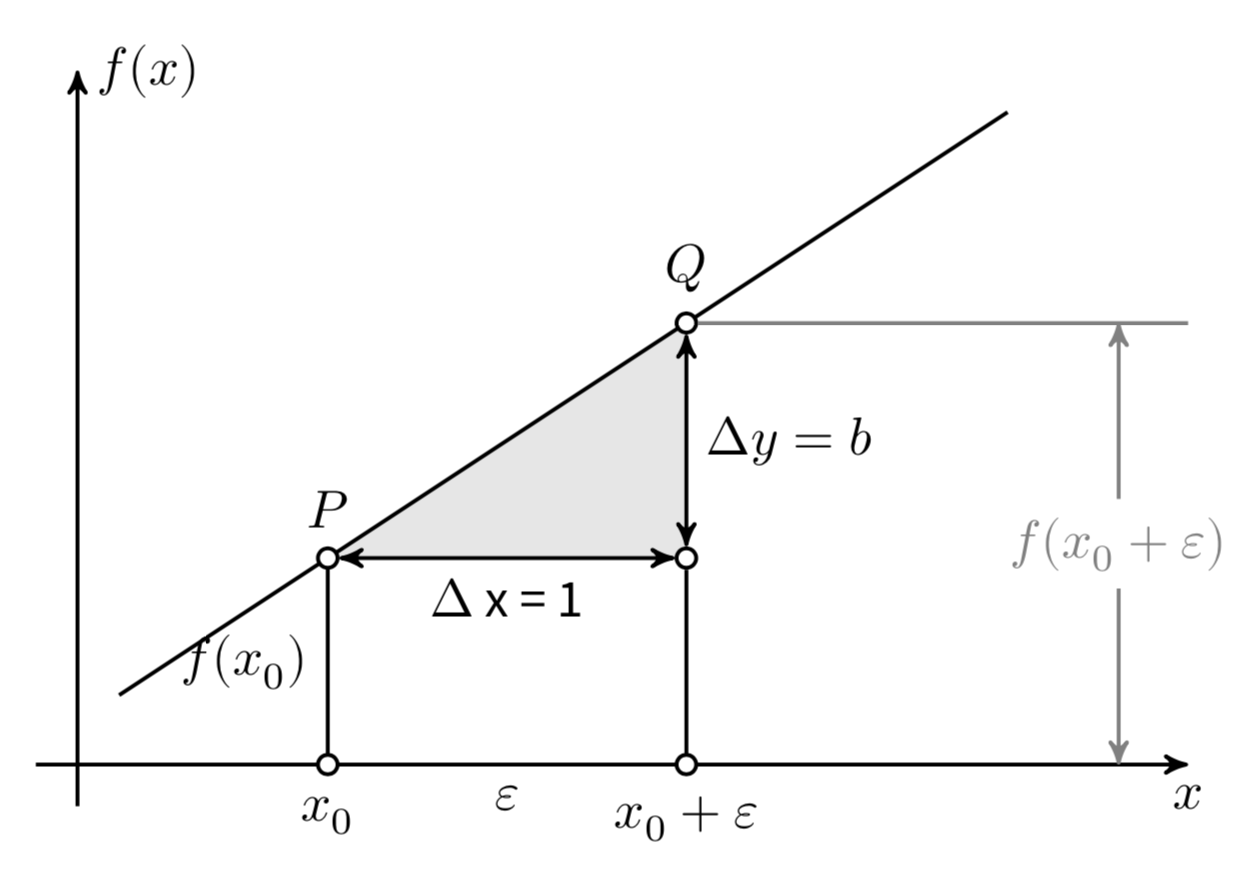
\includegraphics[width=0.7\linewidth]{images/linear_function} 

}

\caption{La funzione lineare $y = a + bx$.}\label{fig:linearfunction}
\end{figure}

\hypertarget{lerrore-di-misurazione}{%
\section{L'errore di misurazione}\label{lerrore-di-misurazione}}

Per descrivere l'associazione tra due variabili, tuttavia, la funzione lineare non è sufficiente. Nel mondo empirico, infatti, la relazione tra variabili non è mai perfettamente lineare. È dunque necessario includere nel modello di regressione anche una componente d'errore, ovvero una componente della \(y\) che non può essere spiegata dal modello lineare. Nel caso di due sole variabili, questo ci conduce alla seguente formulazione del modello di regressione:

\begin{equation}
y = \alpha + \beta x + \varepsilon,
\label{eq:regbivpop}
\end{equation}

laddove i parametri \(\alpha\) e \(\beta\) descrivono l'associazione tra le variabili casuali \(y\) e \(x\), e il termine d'errore \(\varepsilon\) specifica quant'è grande la porzione della variabile \(y\) che non può essere predetta nei termini di una relazione lineare con la \(x\).

Si noti che la \eqref{eq:regbivpop} consente di formulare una predizione, nei termini di un modello lineare, del valore atteso della \(y\) conoscendo \(x\), ovvero

\begin{equation}
\hat{y} = \mathbb{E}(y \mid x) = \alpha + \beta x.
\label{eq:regbivpop2}
\end{equation}

In altri termini, se i parametri del modello (\(\alpha\) e \(\beta\)) sono noti, allora è possibile predire la \(y\) sulla base della nostra conoscenza della \(x\).
Per esempio, se conosciamo la relazione lineare tra quoziente di intelligenza ed aspettativa di vita, allora possiamo prevedere quanto a lungo vivrà una persona sulla base del suo QI. Sì, c'è una relazione lineare tra intelligenza e aspettativa di vita \autocite{hambrick2015research}! Ma quando è accurata la previsione? Ciò dipende dal termine d'errore della \eqref{eq:regbivpop}. L'analisi di regressione fornisce un metodo per rispondere a domande di questo tipo\footnote{Per una discussione sugli aspetti di base della regressione lineare, si veda il \href{https://openintro-ims.netlify.app/model-slr.html}{capitolo 7} di \emph{Introduction to Modern Statistics}.}.

\hypertarget{una-media-per-ciascuna-osservazione}{%
\section{Una media per ciascuna osservazione}\label{una-media-per-ciascuna-osservazione}}

In precedenza abbiamo visto come sia possibile stimare i parametri di un modello bayesiano Normale nel quale le osservazioni sono indipendenti e identicamente distribuite secondo una densità Normale,
\begin{equation}
Y_i \stackrel{i.i.d.}{\sim} \mathcal{N}(\mu, \sigma), \quad i = 1, \dots, n.
\label{eq:normalsamplingmodel}
\end{equation}

Il modello \eqref{eq:normalsamplingmodel} assume che ogni \(Y_i\) sia una realizzazione della stessa \(\mathcal{N}(\mu, \sigma^2)\). Da un punto di vista bayesiano\footnote{Per un'introduzione alla trattazione frequentista dell'analisi di regressione, si veda l'Appendice \ref{least-squares}.}, si assegnano distribuzioni a priori ai parametri \(\mu\) e \(\sigma\), si genera la verosimiglianza in base ai dati osservati e, con queste informazioni, si generano le distribuzione a posteriori dei parametri \autocite{gelman2020regression}:
\begin{align}
Y_i \mid \mu, \sigma & \stackrel{iid}{\sim} \mathcal{N}(\mu, \sigma^2)\notag\\
\mu       & \sim \mathcal{N}(\mu_0, \tau^2) \notag\\
\sigma    & \sim \Cauchy(x_0, \gamma) \notag
\end{align}

È comune però che vengano però registrate altre variabili \(x_i\) che possono essere associate alla risposta di interesse \(y_i\). La variabile \(x_i\) viene chiamata \emph{predittore} (o variabile indipendente) in quanto il ricercatore è tipicamente interessato a predire il valore \(y_i\) a partire da \(x_i\). Come si può estende il modello Normale della \eqref{eq:normalsamplingmodel} per lo studio della possibile relazione tra \(y_i\) e \(x_i\)?

Il modello \eqref{eq:normalsamplingmodel} assume una media \(\mu\) comune per ciascuna osservazione \(Y_i\). Dal momento che desideriamo introdurre una nuova variabile \(x_i\) che assume un valore specifico per ciascuna osservazione \(y_i\), il modello \eqref{eq:normalsamplingmodel} può essere modificato in modo che la media comune \(\mu\) venga sostituita da una media \(\mu_i\) specifica a ciascuna \(i\)-esima osservazione:

\begin{equation}
Y_i \mid \mu_i, \sigma \stackrel{ind}{\sim} \mathcal{N}(\mu_i, \sigma), \quad i = 1, \dots, n.
\label{eq:normalsamplinglinearmodel}
\end{equation}

Si noti che le osservazioni \(Y_1, \dots, Y_n\) non sono più identicamente distribuite poiché hanno medie diverse, ma sono ancora indipendenti come indicato dalla notazione \texttt{ind} posta sopra il simbolo \(\sim\) nella \eqref{eq:normalsamplinglinearmodel}

\hypertarget{relazione-lineare-tra-la-media-y-mid-x-e-il-predittore}{%
\subsection{\texorpdfstring{Relazione lineare tra la media \(y \mid x\) e il predittore}{Relazione lineare tra la media y \textbackslash mid x e il predittore}}\label{relazione-lineare-tra-la-media-y-mid-x-e-il-predittore}}

L'approccio che consente di mettere in relazione un predittore \(x_i\) con la risposta \(Y_i\) è quello di assumere che la media di ciascuna \(Y_i\), ovvero \(\mu_i\), sia una funzione lineare del predittore \(x_i\). Una tale relazione lineare è scritta come

\begin{equation}
\mu_i = \beta_0 + \beta_ 1 x_i, \quad i = 1, \dots, n.
\label{eq:regmodel}
\end{equation}

Nella \eqref{eq:regmodel}, ciascuna \(x_i\) è una costante nota (ecco perché viene usata una lettera minuscola per la \(x\)) e \(\beta_0\) e \(\beta_ 1\) sono parametri incogniti. Questi parametri che rappresentano l'intercetta e la pendenza della retta di regressione sono variabili casuali. Si assegna una distribuzione a priori a \(\beta_0\) e a \(\beta_ 1\) e si esegue l'inferenza riassumendo la distribuzione a posteriori di questi parametri.

In questo modello, la funzione lineare \(\beta_0 + \beta_ 1 x_i\) è interpretata come il valore atteso della \(Y_i\) per ciascun valore \(x_i\), mentre l'intercetta \(\beta_0\) rappresenta il valore atteso della \(Y_i\) quando \(x_i = 0\). Il parametro \(\beta_ 1\) (pendenza) rappresenta invece l'aumento medio della \(Y_i\) quando \(x_i\) aumenta di un'unità. È importante notare che la relazione lineare \eqref{eq:normalsamplinglinearmodel} di parametri \(\beta_0\) e \(\beta_ 1\) descrive l'associazione tra \emph{la media} \(\mu_i\) e il predittore \(x_i\). In altri termini, tale relazione lineare ci fornisce una predizione sul valore medio \(\mu_i\), non sul valore \emph{effettivo} \(Y_i\).

\hypertarget{il-modello-di-regressione-lineare}{%
\subsection{Il modello di regressione lineare}\label{il-modello-di-regressione-lineare}}

Sostituendo la \eqref{eq:regmodel} nel modello \eqref{eq:normalsamplinglinearmodel} otteniamo il modello di regressione lineare:

\begin{equation}
Y_i \mid \beta_0, \beta_ 1, \sigma \stackrel{ind}{\sim} \mathcal{N}(\beta_0 + \beta_ 1 x_i, \sigma), \quad i = 1, \dots, n.
\label{eq:samplinglinearmodel}
\end{equation}

Questo è un caso speciale del modello di campionamento Normale, dove le \(Y_i\) seguono indipendentemente una densità Normale con una media (\(\beta_0 + \beta_ 1 x_i\)) specifica per ciascuna osservazione e con una deviazione standard (\(\sigma\)) comune a tutte le osservazioni. Poiché include un solo predittore (\(x\)), questo modello è comunemente chiamato \emph{modello di regressione lineare semplice}.

In maniera equivalente, il modello \eqref{eq:samplinglinearmodel} può essere formulato come

\begin{equation}
Y_i = \mu_i + \varepsilon_i, \quad i = 1, \dots, n,
\label{eq:samplinglinearmodel2}
\end{equation}

dove la risposta media è \(\mu_i = \beta_0 + \beta_ 1 x_i\) e i residui \(\varepsilon_1, \dots, \varepsilon_n\) sono i.i.d. da una Normale con media 0 e deviazione standard \(\sigma\).

\begin{center}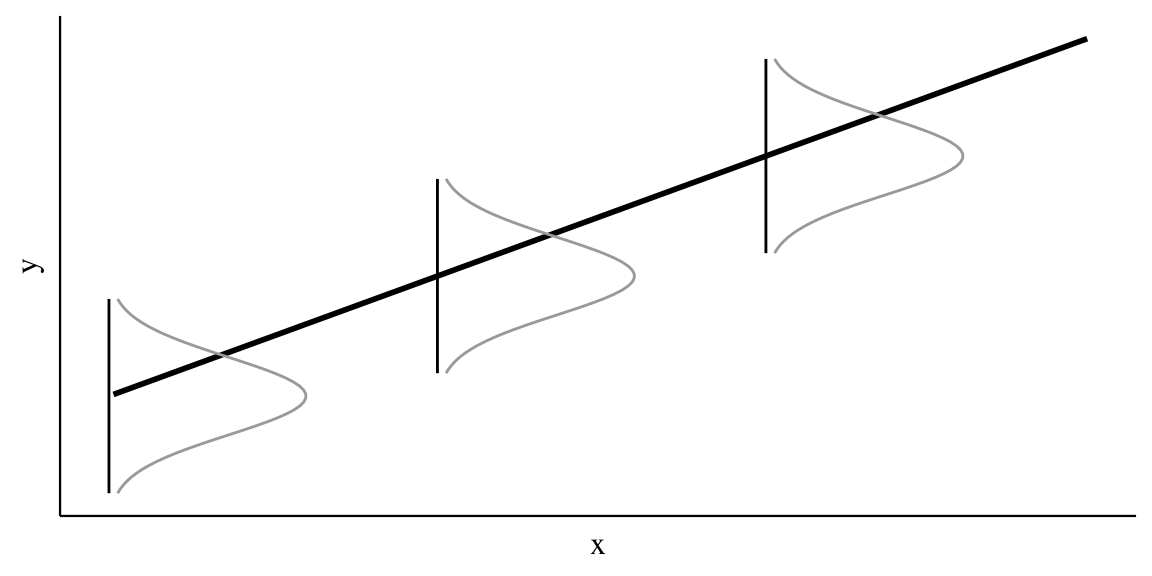
\includegraphics[width=0.8\linewidth]{051_reglin1_files/figure-latex/unnamed-chunk-2-1} \end{center}

Nel modello di regressione lineare, l'osservazione \(Y_i\) è una variabile casuale, il predittore \(x_i\) è una costante fissa, e \(\beta_0\), \(\beta_1\) e \(\sigma\) sono parametri incogniti. Utilizzando il paradigma bayesiano, viene assegnata una distribuzione a priori congiunta a \((\beta_0, \beta_1, \sigma)\). Dopo avere osservato le risposte \(Y_i, i = 1, \dots, n\), l'inferenza procede stimando la distribuzione a posteriori dei parametri.

Nella costruzione di un modello di regressione bayesiano, è importante iniziare dalle basi e procedere un passo alla volta. Sia \(Y\) una variabile di risposta e
sia \(x\) un predittore o un insieme di predittori. È possibile costruire un modello di regressione di \(Y\) su \(x\) applicando i seguenti principi generali:

\begin{itemize}
\tightlist
\item
  Stabilire se \(Y\) è discreto o continuo. Di conseguenza, identificare l'appropriata struttura dei dati (per esempio, Normale, di Poisson, o Binomiale).
\item
  Esprimere la media di \(Y\) come funzione dei predittori \(x\) (per esempio, \(\mu = \beta_0 + \beta_1 x\)).
\item
  Identificare tutti i parametri incogniti del modello (per esempio, \(\mu, \beta_1, \beta_2\)).
\item
  Valutare quali valori che ciascuno di questi parametri potrebbe assumere. Di conseguenza, identificare le distribuzioni a priori appropriate per questi parametri.
\end{itemize}

Nel caso di una variabile \(Y\) continua che segue la legge Normale e un solo predittore, ad esempio, il modello diventa:

\begin{align} 
Y_i \mid \beta_0, \beta_1, \sigma  &\stackrel{ind}{\sim} \mathcal{N}\left(\mu_i, \sigma^2\right) \;\; \text{ con } \;\; \mu_i = \beta_0 + \beta_1 x_i \notag\\
\beta_0  &\sim \mathcal{N}\left(\mu_0, \sigma_0^2 \right)  \notag\\
\beta_1  & \sim \mathcal{N}\left(\mu_1, \sigma_1^2 \right) \notag\\
\sigma & \sim \text{Cauchy}(x_0, \gamma) \; .\notag
\end{align}

Un algoritmo MCMC viene usato per simulare i campioni dalle distribuzioni a posteriori e, mediante tali campioni, si fanno inferenze sulla risposta attesa \(\beta_0 + \beta_1 x\) per ciascuno specifico valore del predittore \(x\). Inoltre, è possibile valutare le dimensioni degli errori di previsione mediante un indice sintetico della densità a posteriori della deviazione standard \(\sigma\).

\hypertarget{considerazioni-conclusive}{%
\section*{Considerazioni conclusive}\label{considerazioni-conclusive}}
\addcontentsline{toc}{section}{Considerazioni conclusive}

Il modello di regressione lineare semplice viene usato per descrivere la
relazione tra due variabili e per determinare il segno e l'intensità di
tale relazione. Inoltre, il modello di regressione ci consente di
prevedere il valore della variabile dipendente in base ad alcuni nuovi
valori della variabile indipendente. Il modello di regressione lineare
semplice è in realtà molto limitato, in quanto descrive soltanto la
relazione tra la variabile dipendente \(y\) e una sola variabile
esplicativa \(x\). Esso diventa molto più utile quando incorpora più
variabili indipendenti. In questo secondo caso, però, i calcoli per la
stima dei coefficienti del modello diventano più complicati. Abbiamo
deciso di iniziare considerando il modello di regressione lineare semplice
perché, in questo caso, sia la logica dell'inferenza sia le procedure di
calcolo sono facilmente maneggiabili. Nel caso più generale, quello del
modello di regressione multipla, la logica dell'inferenza rimarrà
identica a quella discussa qui, ma le procedure di calcolo richiedono
l'uso dell'algebra matriciale. Il modello di regressione multipla può includere sia regressori quantitativi, sia regressori qualitativi, utilizzando un
opportuna schema di codifica. È interessante notare come un modello di
regressione multipla che include una sola variabile esplicativa
quantitativa corrisponde all'analisi della varianza ad una via; un
modello di regressione multipla che include più di una variabile
esplicativa quantitativa corrisponde all'analisi della varianza più vie.
Possiamo qui concludere dicendo che il modello di regressione, nelle sue varie forme e varianti, costituisce la tecnica di analisi dei dati maggiormente usata in psicologia.

\hypertarget{regr-ml}{%
\chapter{Adattare il modello di regressione ai dati}\label{regr-ml}}

\begin{Summary}
In questo Capitolo verranno esposte alcune nozioni matematiche che
stanno alla base dell'inferenza per i modelli di regressione e un po' di
algebra che ci aiuterà a comprendere la stima della regressione lineare.
Spiegheremo anche la logica per l'uso della funzione bayesiana
\texttt{brm()} e la sua connessione con la regressione lineare classica.
\end{Summary}

\hypertarget{minimi-quadrati}{%
\section{Minimi quadrati}\label{minimi-quadrati}}

Nel modello di regressione lineare classico, \(y_i = a + b x_i + \varepsilon_i\), i coefficienti \(a\) e \(b\) sono stimati in modo tale da minimizzare gli errori \(\varepsilon_i\). Se il numero dei dati \(n\) è maggiore di 2, non è generalmente possibile trovare una retta che passi per tutte le osservazioni (\(x, y\)) (sarebbe \(y_i = a + b x_i\), senza errori, per tutti i punti \(i = 1, \dots, n\)). L'obiettivo della stima dei minimi quadrati è quello di scegliere i valori (\(\hat{a}, \hat{b}\)) che minimizzano la somma dei quadrati dei residui,
\begin{equation}
e_i = y_i − (\hat{a} + \hat{b} x_i)\,.
\end{equation}
Distinguiamo tra i residui \(e_i = y_i - (\hat{a} + \hat{b} x_i)\) e gli \emph{errori} \(\varepsilon_i = y_i − (a + b x_i)\). Il modello di regressione è scritto in termini degli errori, ma possiamo solo lavorare con i residui: non possiamo calcolare gli errori perché per farlo sarebbe necessario conoscere i parametri ignoti \(a\) e \(b\).

La somma dei residui quadratici (\emph{residual sum of squares}) è
\begin{equation}
\text{RSS} = \sum_{i=1}^n (y_i = (\hat{a} + \hat{b} x_i))^2\,.
\end{equation}
I coefficienti (\(\hat{a}, \hat{b}\)) che minimizzano RSS sono chiamati stime dei minimi quadrati, o minimi quadrati ordinari (\emph{ordinari least squares}), o stime OLS.

\hypertarget{stima-della-deviazione-standard-dei-residui-sigma}{%
\subsection{\texorpdfstring{Stima della deviazione standard dei residui \(\sigma\)}{Stima della deviazione standard dei residui \textbackslash sigma}}\label{stima-della-deviazione-standard-dei-residui-sigma}}

Nel modello di regressione, gli errori \(\varepsilon_i\) provengono da una distribuzione con media 0 e deviazione standard \(\sigma\): la media è zero per definizione (qualsiasi media diversa da zero viene assorbita nell'intercetta, \(a\)), e la deviazione standard degli errori può essere stimata dai dati. Un modo apparentemente naturale per stimare \(\sigma\) potrebbe essere quello di calcolare la deviazione standard dei residui, \(\sqrt{\frac{1}{n} \sum_{i=1}^n e_i^2} = \sqrt{ \frac{1}{n} \sum_{i=1}^n y_i - (\hat{a} + \hat{b} x_i))^2}\), ma questo approccio finisce per sottostimare \(\sigma\).
La correzione standard di questa sottostima consiste nel sostituire \(n\) con \(n - 2\) al denominatore (la sottrazione di 2 deriva dal fatto che il valore atteso della regressione è stato calcolato utilizzando i due coefficienti nel modello, l'intercetta e la pendenza, i quali sono stati stimati dai dati campionari -- si dice che, in questo modo, abbiamo perso due gradi di libertà). Così facendo otteniamo
\begin{equation}
\hat{\sigma} = \sqrt{\frac{1}{n-2} \sum_{i=1}^n (y_i - (\hat{a} + \hat{b} x_i))^2}\,.
\end{equation}
Quando \(n = 1\) o \(2\) l'equazione precedente è priva di significato, il che ha senso: con solo due osservazioni è possibile adattare esattamente una retta al diagramma di dispersione e quindi non c'è modo di stimare l'errore dai dati.

\hypertarget{calcolare-la-somma-dei-quadrati}{%
\section{Calcolare la somma dei quadrati}\label{calcolare-la-somma-dei-quadrati}}

Seguendo \href{https://github.com/ASKurz/Working-through-Regression-and-other-stories/blob/main/08.Rmd}{Solomon Kurz}, creiamo una funzione per calcolare la somma dei quadrati per diversi valori di \(a\) e \(b\):

\begin{Shaded}
\begin{Highlighting}[]
\NormalTok{rss }\OtherTok{\textless{}{-}} \ControlFlowTok{function}\NormalTok{(x, y, a, b) \{  }
  \CommentTok{\# x and y are vectors, }
  \CommentTok{\# a and b are scalars }
\NormalTok{  resid }\OtherTok{\textless{}{-}}\NormalTok{ y }\SpecialCharTok{{-}}\NormalTok{ (a }\SpecialCharTok{+}\NormalTok{ b }\SpecialCharTok{*}\NormalTok{ x)}
  \FunctionTok{return}\NormalTok{(}\FunctionTok{sum}\NormalTok{(resid}\SpecialCharTok{\^{}}\DecValTok{2}\NormalTok{))}
\NormalTok{  \}}
\end{Highlighting}
\end{Shaded}

Useremo i dati \ldots.

\begin{Shaded}
\begin{Highlighting}[]
\NormalTok{df }\OtherTok{\textless{}{-}} \FunctionTok{read.dta}\NormalTok{(}\FunctionTok{here}\NormalTok{(}\StringTok{"data"}\NormalTok{, }\StringTok{"kidiq.dta"}\NormalTok{))}
\FunctionTok{head}\NormalTok{(df)}
\CommentTok{\#\textgreater{}   kid\_score mom\_hs mom\_iq mom\_work mom\_age}
\CommentTok{\#\textgreater{} 1        65      1  121.1        4      27}
\CommentTok{\#\textgreater{} 2        98      1   89.4        4      25}
\CommentTok{\#\textgreater{} 3        85      1  115.4        4      27}
\CommentTok{\#\textgreater{} 4        83      1   99.4        3      25}
\CommentTok{\#\textgreater{} 5       115      1   92.7        4      27}
\CommentTok{\#\textgreater{} 6        98      0  107.9        1      18}
\end{Highlighting}
\end{Shaded}

Nell'esempio, \texttt{kid\_score} è la variabile \(y\) e \texttt{mom\_iq} è il predittore. Le stime dei minimi quadrati sono fornite dalla funzione \texttt{lm()}:

\begin{Shaded}
\begin{Highlighting}[]
\NormalTok{fm }\OtherTok{\textless{}{-}} \FunctionTok{lm}\NormalTok{(kid\_score }\SpecialCharTok{\textasciitilde{}}\NormalTok{ mom\_iq, }\AttributeTok{data =}\NormalTok{ df)}
\NormalTok{fm }\SpecialCharTok{\%\textgreater{}\%}
  \FunctionTok{tidy}\NormalTok{() }\SpecialCharTok{\%\textgreater{}\%} 
  \FunctionTok{filter}\NormalTok{(term }\SpecialCharTok{==} \FunctionTok{c}\NormalTok{(}\StringTok{"(Intercept)"}\NormalTok{, }\StringTok{"mom\_iq"}\NormalTok{)) }\SpecialCharTok{\%\textgreater{}\%} 
  \FunctionTok{pull}\NormalTok{(estimate)}
\CommentTok{\#\textgreater{} [1] 25.80  0.61}
\end{Highlighting}
\end{Shaded}

Calcoliamo la somma dei residui quadratici in base al modello di regressione \(\hat{y}_i = 25.8 + 0.61 x_i\):

\begin{Shaded}
\begin{Highlighting}[]
\FunctionTok{rss}\NormalTok{(df}\SpecialCharTok{$}\NormalTok{mom\_iq, df}\SpecialCharTok{$}\NormalTok{kid\_score, }\FloatTok{25.8}\NormalTok{, }\FloatTok{0.61}\NormalTok{)}
\CommentTok{\#\textgreater{} [1] 144137}
\end{Highlighting}
\end{Shaded}

Esploriamo ora i valori assunti da \(rss\) per diversi valori di \(a\) e \(b\). Per iniziare, utilizziamo un vettore di valori \texttt{a}, mantenendo costante \texttt{b\ =\ 0.61}.

\begin{Shaded}
\begin{Highlighting}[]
\CommentTok{\# set the global plotting theme}
\CommentTok{\# theme\_set(theme\_linedraw() +}
\CommentTok{\#             theme(panel.grid = element\_blank()))}
\CommentTok{\# simulate}
\FunctionTok{tibble}\NormalTok{(}\AttributeTok{a =} \FunctionTok{seq}\NormalTok{(}\DecValTok{20}\NormalTok{, }\DecValTok{30}\NormalTok{, }\AttributeTok{length.out =} \DecValTok{30}\NormalTok{)) }\SpecialCharTok{\%\textgreater{}\%} 
  \FunctionTok{mutate}\NormalTok{(}
    \AttributeTok{rss =} \FunctionTok{map\_dbl}\NormalTok{(}
\NormalTok{      a, }
\NormalTok{      rss, }
      \AttributeTok{x =}\NormalTok{ df}\SpecialCharTok{$}\NormalTok{mom\_iq, }
      \AttributeTok{y =}\NormalTok{ df}\SpecialCharTok{$}\NormalTok{kid\_score,  }
      \AttributeTok{b =} \FloatTok{0.61}\NormalTok{)}
\NormalTok{    ) }\SpecialCharTok{\%\textgreater{}\%} 
  
  \CommentTok{\# plot}
  \FunctionTok{ggplot}\NormalTok{(}\FunctionTok{aes}\NormalTok{(}\AttributeTok{x =}\NormalTok{ a, }\AttributeTok{y =}\NormalTok{ rss)) }\SpecialCharTok{+}
  \FunctionTok{geom\_point}\NormalTok{() }\SpecialCharTok{+}
  \FunctionTok{labs}\NormalTok{(}\AttributeTok{subtitle =} \StringTok{"Il valore b è tenuto costante (b = 0.61)"}\NormalTok{) }
\end{Highlighting}
\end{Shaded}

\begin{center}\includegraphics[width=0.8\linewidth]{052_reglin2_files/figure-latex/unnamed-chunk-7-1} \end{center}

Ora variamo sia \texttt{a} che \texttt{b}, facendo assumere a ciascun parametro un insieme di valori in un intevallo, e rappresentiamo i risultati in una heat map che rappresenta l'intensitè di \texttt{rss} in funzione dei valori \texttt{a} e \texttt{b}.

\begin{Shaded}
\begin{Highlighting}[]
\NormalTok{d }\OtherTok{\textless{}{-}}
  \FunctionTok{crossing}\NormalTok{(}\AttributeTok{a =} \FunctionTok{seq}\NormalTok{(}\SpecialCharTok{{-}}\DecValTok{20}\NormalTok{, }\DecValTok{70}\NormalTok{, }\AttributeTok{length.out =} \DecValTok{400}\NormalTok{),}
           \AttributeTok{b =} \FunctionTok{seq}\NormalTok{(}\SpecialCharTok{{-}}\FloatTok{0.2}\NormalTok{, }\FloatTok{1.4}\NormalTok{, }\AttributeTok{length.out =} \DecValTok{400}\NormalTok{)) }\SpecialCharTok{\%\textgreater{}\%} 
  \FunctionTok{mutate}\NormalTok{(}\AttributeTok{rss =} \FunctionTok{map2\_dbl}\NormalTok{(a, b, rss, }\AttributeTok{x =}\NormalTok{ df}\SpecialCharTok{$}\NormalTok{mom\_iq, }\AttributeTok{y =}\NormalTok{ df}\SpecialCharTok{$}\NormalTok{kid\_score))}
\NormalTok{d }\SpecialCharTok{\%\textgreater{}\%}
  \FunctionTok{ggplot}\NormalTok{(}\FunctionTok{aes}\NormalTok{(}\AttributeTok{x =}\NormalTok{ a, }\AttributeTok{y =}\NormalTok{ b, }\AttributeTok{fill =}\NormalTok{ rss)) }\SpecialCharTok{+}
  \FunctionTok{geom\_tile}\NormalTok{() }\SpecialCharTok{+}
  \FunctionTok{scale\_fill\_viridis\_c}\NormalTok{(}\StringTok{"RSS"}\NormalTok{, }\AttributeTok{option =} \StringTok{"A"}\NormalTok{) }\SpecialCharTok{+}
  \FunctionTok{scale\_x\_continuous}\NormalTok{(}\AttributeTok{expand =} \FunctionTok{c}\NormalTok{(}\DecValTok{0}\NormalTok{, }\DecValTok{0}\NormalTok{)) }\SpecialCharTok{+}
  \FunctionTok{scale\_y\_continuous}\NormalTok{(}\AttributeTok{expand =} \FunctionTok{c}\NormalTok{(}\DecValTok{0}\NormalTok{, }\DecValTok{0}\NormalTok{))}
\end{Highlighting}
\end{Shaded}

\begin{center}\includegraphics[width=0.8\linewidth]{052_reglin2_files/figure-latex/unnamed-chunk-8-1} \end{center}

Poiché la stima dei minimi quadrati enfatizza il valore RSS minimo, la soluzione che cerchiamo corrisponde alle combinazione di \texttt{a} e \texttt{b} nell'intervallo più scuro rappresentato nella figura. Tra gli \texttt{a} e \texttt{b} che abbiamo preso in considerazione, la coppia di valori a cui è associato il minimo valore \texttt{rss} si trova nel modo seguente:

\begin{Shaded}
\begin{Highlighting}[]
\NormalTok{d }\SpecialCharTok{\%\textgreater{}\%} 
  \FunctionTok{arrange}\NormalTok{(rss) }\SpecialCharTok{\%\textgreater{}\%} 
  \FunctionTok{slice}\NormalTok{(}\DecValTok{1}\NormalTok{)}
\CommentTok{\#\textgreater{} \# A tibble: 1 x 3}
\CommentTok{\#\textgreater{}       a     b     rss}
\CommentTok{\#\textgreater{}   \textless{}dbl\textgreater{} \textless{}dbl\textgreater{}   \textless{}dbl\textgreater{}}
\CommentTok{\#\textgreater{} 1  25.8 0.610 144137.}
\end{Highlighting}
\end{Shaded}

Si noti che i valori trovati in questo modo corrispondono alla soluzione fornita nell'output della funzione \texttt{lm()}.

\hypertarget{massima-verosimiglianza}{%
\section{Massima verosimiglianza}\label{massima-verosimiglianza}}

Se gli errori del modello lineare sono indipendenti e distribuiti normalmente, in modo che \(y_i \sim \mathcal{N}(a + b x_i, \sigma^2)\) per ogni \(i\), allora la stima ai minimi quadrati di (\texttt{a}, \texttt{b}) è anche la stima di massima verosimiglianza. La \emph{funzione di verosimiglianza} in un modello di regressione è definita come la densità di probabilità delle osservazioni dati i parametri e i predittori; quindi, in questo esempio,
\[
 p(y \mid a, b, \sigma, x) = \prod_{i=1}^n \mathcal{N}(y_i \mid a + b x_i, \sigma^2),
 \]

dove \(\mathcal{N}(\cdot | \cdot, \cdot)\) è la funzione di densità di probabilità normale,
\[
\mathcal{N}(y \mid \mu, \sigma^2) = \frac{1}{\sqrt{2 \pi \sigma}} \exp \left(-\frac{1}{2} \left( \frac{y - \mu}{\sigma} \right)^2 \right).
\]

Un studio della funzione precedente rivela che la massimizzazione della verosimiglianza richiede la minimizzazione della somma dei quadrati dei residui; quindi la stima dei minimi quadrati \(\hat{\beta} = (\hat{a}, \hat{b})\) può essere vista come una stima di massima verosimiglianza nel modello normale:

\begin{Shaded}
\begin{Highlighting}[]
\NormalTok{ll }\OtherTok{\textless{}{-}} \ControlFlowTok{function}\NormalTok{(x, y, a, b) \{}
\NormalTok{  resid }\OtherTok{\textless{}{-}}\NormalTok{ y }\SpecialCharTok{{-}}\NormalTok{ (a }\SpecialCharTok{+}\NormalTok{ b }\SpecialCharTok{*}\NormalTok{ x)}
\NormalTok{  sigma }\OtherTok{\textless{}{-}} \FunctionTok{sqrt}\NormalTok{(}\FunctionTok{sum}\NormalTok{(resid}\SpecialCharTok{\^{}}\DecValTok{2}\NormalTok{) }\SpecialCharTok{/} \FunctionTok{length}\NormalTok{(x))}
\NormalTok{  d }\OtherTok{\textless{}{-}} \FunctionTok{dnorm}\NormalTok{(y, }\AttributeTok{mean =}\NormalTok{ a }\SpecialCharTok{+}\NormalTok{ b }\SpecialCharTok{*}\NormalTok{ x, }\AttributeTok{sd =}\NormalTok{ sigma, }\AttributeTok{log =} \ConstantTok{TRUE}\NormalTok{)}
  \FunctionTok{tibble}\NormalTok{(}\AttributeTok{sigma =}\NormalTok{ sigma, }\AttributeTok{ll =} \FunctionTok{sum}\NormalTok{(d))}
\NormalTok{\}}
\end{Highlighting}
\end{Shaded}

Calcoliamo dunque le stime di verosimiglianza logaritmica per varie combinazioni di (\texttt{a}, \texttt{b}), date due colonne di dati, \texttt{x} e \texttt{y}. La funzione resituisce anche il valore \(\hat{\sigma}\).

\begin{Shaded}
\begin{Highlighting}[]
\NormalTok{d }\OtherTok{\textless{}{-}}
  \FunctionTok{crossing}\NormalTok{(}\AttributeTok{a =} \FunctionTok{seq}\NormalTok{(}\SpecialCharTok{{-}}\DecValTok{20}\NormalTok{, }\DecValTok{70}\NormalTok{, }\AttributeTok{length.out =} \DecValTok{200}\NormalTok{),}
           \AttributeTok{b =} \FunctionTok{seq}\NormalTok{(}\SpecialCharTok{{-}}\FloatTok{0.2}\NormalTok{, }\FloatTok{1.4}\NormalTok{, }\AttributeTok{length.out =} \DecValTok{200}\NormalTok{)) }\SpecialCharTok{\%\textgreater{}\%} 
  \FunctionTok{mutate}\NormalTok{(}\AttributeTok{ll =} \FunctionTok{map2}\NormalTok{(a, b, ll, }\AttributeTok{x =}\NormalTok{ df}\SpecialCharTok{$}\NormalTok{mom\_iq, }\AttributeTok{y =}\NormalTok{ df}\SpecialCharTok{$}\NormalTok{kid\_score)) }\SpecialCharTok{\%\textgreater{}\%} 
  \FunctionTok{unnest}\NormalTok{(ll)}
\NormalTok{p1 }\OtherTok{\textless{}{-}}
\NormalTok{  d }\SpecialCharTok{\%\textgreater{}\%}
  \FunctionTok{ggplot}\NormalTok{(}\FunctionTok{aes}\NormalTok{(}\AttributeTok{x =}\NormalTok{ a, }\AttributeTok{y =}\NormalTok{ b, }\AttributeTok{fill =}\NormalTok{ ll)) }\SpecialCharTok{+}
  \FunctionTok{geom\_tile}\NormalTok{() }\SpecialCharTok{+}
  \FunctionTok{scale\_fill\_viridis\_c}\NormalTok{(}\AttributeTok{option =} \StringTok{"A"}\NormalTok{, }\AttributeTok{breaks =} \ConstantTok{NULL}\NormalTok{) }\SpecialCharTok{+}
  \FunctionTok{scale\_x\_continuous}\NormalTok{(}\AttributeTok{expand =} \FunctionTok{c}\NormalTok{(}\DecValTok{0}\NormalTok{, }\DecValTok{0}\NormalTok{)) }\SpecialCharTok{+}
  \FunctionTok{scale\_y\_continuous}\NormalTok{(}\AttributeTok{expand =} \FunctionTok{c}\NormalTok{(}\DecValTok{0}\NormalTok{, }\DecValTok{0}\NormalTok{)) }\SpecialCharTok{+}
  \FunctionTok{labs}\NormalTok{(}\AttributeTok{subtitle =} \StringTok{"Verosimiglianza, p(a, b | y)"}\NormalTok{)}
\NormalTok{p1}
\end{Highlighting}
\end{Shaded}

\begin{center}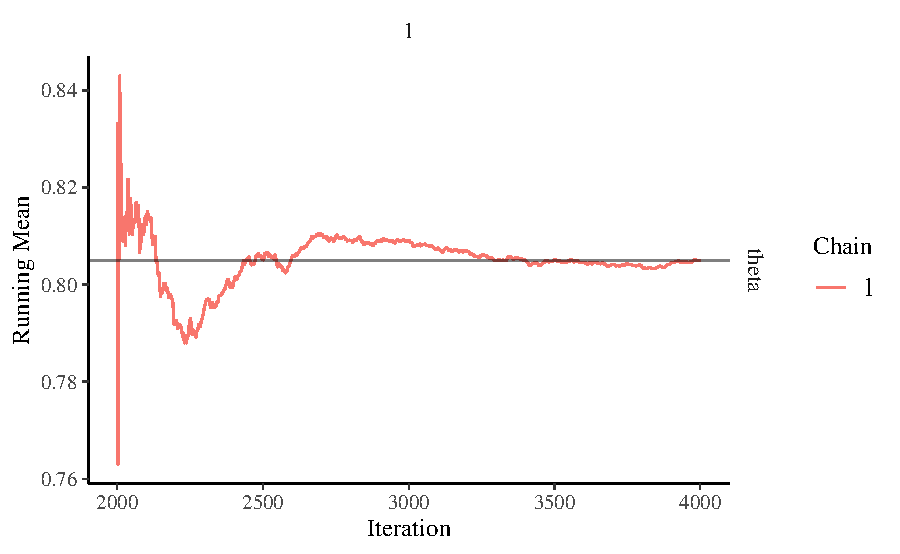
\includegraphics[width=0.8\linewidth]{052_reglin2_files/figure-latex/unnamed-chunk-11-1} \end{center}

Le stime di \(\hat{a}, \hat{b}\) ottenute mediante il metodo di massima verosimiglianza sono:

\begin{Shaded}
\begin{Highlighting}[]
\NormalTok{d }\SpecialCharTok{\%\textgreater{}\%} 
  \FunctionTok{arrange}\NormalTok{(}\FunctionTok{desc}\NormalTok{(ll)) }\SpecialCharTok{\%\textgreater{}\%} 
  \FunctionTok{slice}\NormalTok{(}\DecValTok{1}\NormalTok{)}
\CommentTok{\#\textgreater{} \# A tibble: 1 x 4}
\CommentTok{\#\textgreater{}       a     b sigma     ll}
\CommentTok{\#\textgreater{}   \textless{}dbl\textgreater{} \textless{}dbl\textgreater{} \textless{}dbl\textgreater{}  \textless{}dbl\textgreater{}}
\CommentTok{\#\textgreater{} 1  25.7 0.612  18.2 {-}1876.}
\end{Highlighting}
\end{Shaded}

\hypertarget{inferenza-bayesiana}{%
\subsection{Inferenza bayesiana}\label{inferenza-bayesiana}}

Usiamo ora la funzione \texttt{brms::brm()} per eseguire l'analisi mediante un approccio bayesiano:

\begin{Shaded}
\begin{Highlighting}[]
\NormalTok{m }\OtherTok{\textless{}{-}}
  \FunctionTok{brm}\NormalTok{(}
\NormalTok{    kid\_score }\SpecialCharTok{\textasciitilde{}}\NormalTok{ mom\_iq,}
    \AttributeTok{data =}\NormalTok{ df, }
    \AttributeTok{backend =} \StringTok{"cmdstan"}\NormalTok{,}
    \AttributeTok{refresh =} \DecValTok{0}
\NormalTok{  )}
\CommentTok{\#\textgreater{} Running MCMC with 4 chains, at most 8 in parallel...}
\CommentTok{\#\textgreater{} }
\CommentTok{\#\textgreater{} Chain 1 finished in 0.0 seconds.}
\CommentTok{\#\textgreater{} Chain 2 finished in 0.0 seconds.}
\CommentTok{\#\textgreater{} Chain 3 finished in 0.0 seconds.}
\CommentTok{\#\textgreater{} Chain 4 finished in 0.0 seconds.}
\CommentTok{\#\textgreater{} }
\CommentTok{\#\textgreater{} All 4 chains finished successfully.}
\CommentTok{\#\textgreater{} Mean chain execution time: 0.0 seconds.}
\CommentTok{\#\textgreater{} Total execution time: 0.3 seconds.}
\end{Highlighting}
\end{Shaded}

Utilizzando i coefficienti calcolati da \texttt{brms::brm()}, aggiungiamo la stima della retta di regressione al diagramma di dispersione dei dati:

\begin{Shaded}
\begin{Highlighting}[]
\NormalTok{df }\SpecialCharTok{\%\textgreater{}\%} 
  \FunctionTok{ggplot}\NormalTok{(}\FunctionTok{aes}\NormalTok{(}\AttributeTok{x =}\NormalTok{ mom\_iq, }\AttributeTok{y =}\NormalTok{ kid\_score)) }\SpecialCharTok{+}
  \FunctionTok{geom\_point}\NormalTok{() }\SpecialCharTok{+}
  \FunctionTok{geom\_abline}\NormalTok{(}
    \AttributeTok{intercept =} \FunctionTok{fixef}\NormalTok{(m, }\AttributeTok{robust =} \ConstantTok{TRUE}\NormalTok{)[}\DecValTok{1}\NormalTok{, }\DecValTok{1}\NormalTok{], }
    \AttributeTok{slope =} \FunctionTok{fixef}\NormalTok{(m, }\AttributeTok{robust =} \ConstantTok{TRUE}\NormalTok{)[}\DecValTok{2}\NormalTok{, }\DecValTok{1}\NormalTok{],}
    \AttributeTok{size =} \DecValTok{1}\SpecialCharTok{/}\DecValTok{3}
\NormalTok{  ) }\SpecialCharTok{+}
  \FunctionTok{annotate}\NormalTok{(}
    \AttributeTok{geom =} \StringTok{"text"}\NormalTok{,}
    \AttributeTok{x =} \DecValTok{130}\NormalTok{, }\AttributeTok{y =} \DecValTok{30}\NormalTok{,}
    \AttributeTok{label =} \FunctionTok{expression}\NormalTok{(y }\SpecialCharTok{==} \FloatTok{25.7} \SpecialCharTok{+} \FloatTok{0.61} \SpecialCharTok{*}\NormalTok{ x)}
\NormalTok{  ) }\SpecialCharTok{+}
  \FunctionTok{labs}\NormalTok{(}
    \AttributeTok{subtitle =} \StringTok{"Dati e retta di regressione"}\NormalTok{,}
    \AttributeTok{x =} \StringTok{"x"}\NormalTok{,}
    \AttributeTok{y =} \StringTok{"y"}
\NormalTok{  ) }
\end{Highlighting}
\end{Shaded}

\begin{center}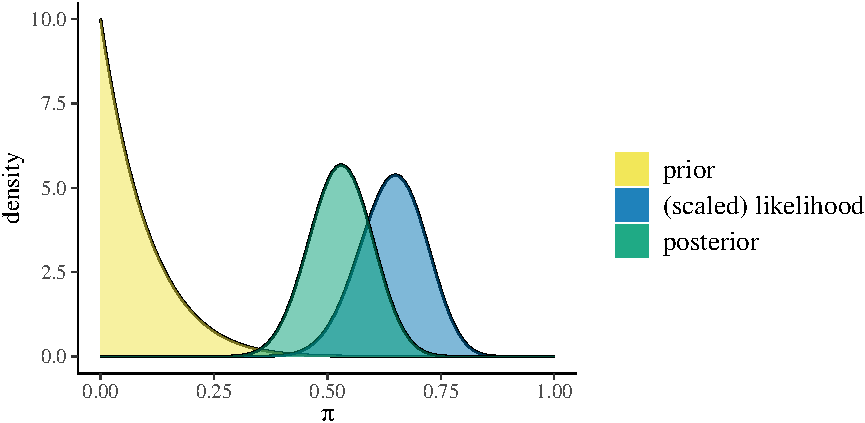
\includegraphics[width=0.8\linewidth]{052_reglin2_files/figure-latex/unnamed-chunk-14-1} \end{center}

La funzione \texttt{brms::posterior\_samples()} consente di estrarre molti campioni dalla distribuzione a posteriori del modello \texttt{m}. In questo modo otteniamo un vettore di valori per ciascuno dei tre parametri, i quali, in questo output sono chiamati \texttt{b\_Intercept}, \texttt{b\_mom\_iq} e \texttt{sigma}. Abbiamo quindi usato \texttt{slice\_sample()} per ottenere un sottoinsieme casuale di 50 righe. Per semplicità, qui ne stampiamo solo 5.

\begin{Shaded}
\begin{Highlighting}[]
\FunctionTok{set.seed}\NormalTok{(}\DecValTok{8}\NormalTok{)}

\FunctionTok{posterior\_samples}\NormalTok{(m) }\SpecialCharTok{\%\textgreater{}\%} 
  \FunctionTok{slice\_sample}\NormalTok{(}\AttributeTok{n =} \DecValTok{5}\NormalTok{)}
\CommentTok{\#\textgreater{}   b\_Intercept b\_mom\_iq sigma Intercept  lp\_\_}
\CommentTok{\#\textgreater{} 1        18.7    0.671  19.2      85.8 {-}1883}
\CommentTok{\#\textgreater{} 2        20.4    0.663  17.9      86.7 {-}1881}
\CommentTok{\#\textgreater{} 3        33.3    0.546  18.5      87.8 {-}1882}
\CommentTok{\#\textgreater{} 4        25.5    0.620  18.3      87.5 {-}1881}
\CommentTok{\#\textgreater{} 5        29.0    0.577  18.2      86.7 {-}1881}
\end{Highlighting}
\end{Shaded}

Possiamo interpretare i valori \texttt{b\_Intercept}, \texttt{b\_mom\_iq} come un insieme di valori credibili per i parametri \(a\) e \(b\). Dati questi valori credibili per i parametri del modello di regressione, possiamo aggiungere al diagramma a dispersione 50 stime possibili della retta di regressione, alla luce dei dati osservati.

\begin{Shaded}
\begin{Highlighting}[]
\FunctionTok{set.seed}\NormalTok{(}\DecValTok{8}\NormalTok{)}

\FunctionTok{posterior\_samples}\NormalTok{(m) }\SpecialCharTok{\%\textgreater{}\%} 
  \FunctionTok{slice\_sample}\NormalTok{(}\AttributeTok{n =} \DecValTok{50}\NormalTok{) }\SpecialCharTok{\%\textgreater{}\%} 
  
  \FunctionTok{ggplot}\NormalTok{() }\SpecialCharTok{+}
  \FunctionTok{geom\_abline}\NormalTok{(}
    \FunctionTok{aes}\NormalTok{(}\AttributeTok{intercept =}\NormalTok{ b\_Intercept, }\AttributeTok{slope =}\NormalTok{ b\_mom\_iq),}
        \AttributeTok{size =} \DecValTok{1}\SpecialCharTok{/}\DecValTok{4}\NormalTok{, }\AttributeTok{alpha =} \DecValTok{1}\SpecialCharTok{/}\DecValTok{2}\NormalTok{, }\AttributeTok{color =} \StringTok{"grey25"}\NormalTok{) }\SpecialCharTok{+}
  \FunctionTok{geom\_point}\NormalTok{(}
    \AttributeTok{data =}\NormalTok{ df,}
    \FunctionTok{aes}\NormalTok{(}\AttributeTok{x =}\NormalTok{ mom\_iq, }\AttributeTok{y =}\NormalTok{ kid\_score)}
\NormalTok{  ) }\SpecialCharTok{+}
  \FunctionTok{labs}\NormalTok{(}
    \AttributeTok{subtitle =} \StringTok{"Dati e possibili rette di regressione"}\NormalTok{,}
    \AttributeTok{x =} \StringTok{"x"}\NormalTok{,}
    \AttributeTok{y =} \StringTok{"y"}
\NormalTok{  ) }
\end{Highlighting}
\end{Shaded}

\begin{center}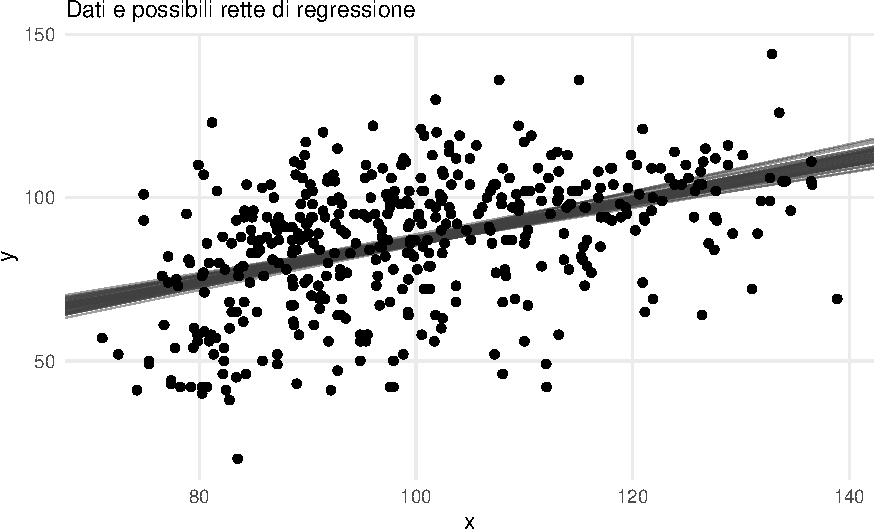
\includegraphics[width=0.8\linewidth]{052_reglin2_files/figure-latex/unnamed-chunk-16-1} \end{center}

I minimi quadrati o la massima verosimiglianza trovano i parametri che meglio si adattano ai dati (secondo un criterio prestabilito), ma senza altrimenti vincolare o guidare l'adattamento. Ma di solito abbiamo informazioni preliminari sui parametri del modello. L'inferenza bayesiana produce un compromesso tra informazioni a priori e i dati, moltiplicando la verosimiglianza con una distribuzione a priori che codifica probabilisticamente le informazioni esterne sui parametri. Il prodotto della verosimiglianza \(p(y \mid a, b, \sigma)\) e della distribuzione a priori è chiamato \emph{distribuzione a posteriori} e, dopo aver visto i dati, riassume la nostra credenza sui valori dei parametri.

La soluzione dei minimi quadrati fornisce una stima puntuale dei coefficienti che producono il miglior adattamento complessivo ai dati. Per un modello bayesiano, la corrispondente stima puntuale è la moda a posteriori, la quale fornisce il miglior adattamento complessivo ai dati e alla distribuzione a priori. La stima dei minimi quadrati o di massima verosimiglianza è la moda a posteriori corrispondente al modello bayesiano che utilizza una distribuzione a priori uniforme.

Ma non vogliamo solo una stima puntuale; vogliamo anche una misura dell'incertezza della stima. La figura precedente fornisce, in forma grafica, una descrizione di tale incertezza.

Gli intervalli di credibilità al 95\% si ottengono nel modo seguente:

\begin{Shaded}
\begin{Highlighting}[]
\FunctionTok{print}\NormalTok{(m, }\AttributeTok{robust =} \ConstantTok{TRUE}\NormalTok{)}
\CommentTok{\#\textgreater{}  Family: gaussian }
\CommentTok{\#\textgreater{}   Links: mu = identity; sigma = identity }
\CommentTok{\#\textgreater{} Formula: kid\_score \textasciitilde{} mom\_iq }
\CommentTok{\#\textgreater{}    Data: df (Number of observations: 434) }
\CommentTok{\#\textgreater{}   Draws: 4 chains, each with iter = 1000; warmup = 0; thin = 1;}
\CommentTok{\#\textgreater{}          total post{-}warmup draws = 4000}
\CommentTok{\#\textgreater{} }
\CommentTok{\#\textgreater{} Population{-}Level Effects: }
\CommentTok{\#\textgreater{}           Estimate Est.Error l{-}95\% CI u{-}95\% CI Rhat Bulk\_ESS Tail\_ESS}
\CommentTok{\#\textgreater{} Intercept    25.83      5.80    14.44    37.47 1.00     3329     3005}
\CommentTok{\#\textgreater{} mom\_iq        0.61      0.06     0.49     0.72 1.00     3310     3009}
\CommentTok{\#\textgreater{} }
\CommentTok{\#\textgreater{} Family Specific Parameters: }
\CommentTok{\#\textgreater{}       Estimate Est.Error l{-}95\% CI u{-}95\% CI Rhat Bulk\_ESS Tail\_ESS}
\CommentTok{\#\textgreater{} sigma    18.26      0.61    17.13    19.53 1.00     3824     3105}
\CommentTok{\#\textgreater{} }
\CommentTok{\#\textgreater{} Draws were sampled using sample(hmc). For each parameter, Bulk\_ESS}
\CommentTok{\#\textgreater{} and Tail\_ESS are effective sample size measures, and Rhat is the potential}
\CommentTok{\#\textgreater{} scale reduction factor on split chains (at convergence, Rhat = 1).}
\end{Highlighting}
\end{Shaded}

In alternativa, è possibile usare la funzione \texttt{posterior\_interval()}:

\begin{Shaded}
\begin{Highlighting}[]
\FunctionTok{posterior\_interval}\NormalTok{(m)}
\CommentTok{\#\textgreater{}                  2.5\%     97.5\%}
\CommentTok{\#\textgreater{} b\_Intercept    14.445    37.471}
\CommentTok{\#\textgreater{} b\_mom\_iq        0.495     0.722}
\CommentTok{\#\textgreater{} sigma          17.132    19.529}
\CommentTok{\#\textgreater{} Intercept      85.119    88.563}
\CommentTok{\#\textgreater{} lp\_\_        {-}1885.190 {-}1880.580}
\end{Highlighting}
\end{Shaded}

\hypertarget{reg-lin-stan}{%
\chapter{Regressione lineare in Stan}\label{reg-lin-stan}}

\hypertarget{la-specificazione-del-modello-in-linguaggio-stan}{%
\section{La specificazione del modello in linguaggio Stan}\label{la-specificazione-del-modello-in-linguaggio-stan}}

Obiettivo di questo Capitolo è illustrare come svolgere l'analisi di regressione bayesiana usando il linguaggio Stan.\footnote{Una descrizione dell'approccio frequentista all'analisi di regressione è fornita nell'Appendice \ref{regr-lin-frequentista}.} Per fare un esempio concreto useremo un famoso dataset chiamato \texttt{kidiq} \autocite{gelman2020regression} che riporta i dati di un'indagine del 2007 su un campione di donne americane adulte e sui loro bambini di età compres tra i 3 e i 4 anni. I dati sono costituiti da 434 osservazioni e 4 variabili:

\begin{itemize}
\tightlist
\item
  \texttt{kid\_score}: QI del bambino; è il punteggio totale del \emph{Peabody Individual Achievement Test} (PIAT) costituito dalla somma dei punteggi di tre sottoscale (Mathematics, Reading comprehension, Reading recognition);
\item
  \texttt{mom\_hs}: variabile dicotomica (0 or 1) che indica se la madre del bambino ha completato le scuole superiori (1) oppure no (0);
\item
  \texttt{mom\_iq}: QI della madre;
\item
  \texttt{mom\_age}: età della madre.
\end{itemize}

Leggiamo i dati in \R:

\begin{Shaded}
\begin{Highlighting}[]
\FunctionTok{library}\NormalTok{(}\StringTok{"foreign"}\NormalTok{)}
\NormalTok{df }\OtherTok{\textless{}{-}} \FunctionTok{read.dta}\NormalTok{(}\FunctionTok{here}\NormalTok{(}\StringTok{"data"}\NormalTok{, }\StringTok{"kidiq.dta"}\NormalTok{))}
\FunctionTok{head}\NormalTok{(df)}
\CommentTok{\#\textgreater{}   kid\_score mom\_hs mom\_iq mom\_work mom\_age}
\CommentTok{\#\textgreater{} 1        65      1  121.1        4      27}
\CommentTok{\#\textgreater{} 2        98      1   89.4        4      25}
\CommentTok{\#\textgreater{} 3        85      1  115.4        4      27}
\CommentTok{\#\textgreater{} 4        83      1   99.4        3      25}
\CommentTok{\#\textgreater{} 5       115      1   92.7        4      27}
\CommentTok{\#\textgreater{} 6        98      0  107.9        1      18}
\end{Highlighting}
\end{Shaded}

Calcoliamo alcune statistiche descrittive:

\begin{Shaded}
\begin{Highlighting}[]
\FunctionTok{summary}\NormalTok{(df)}
\CommentTok{\#\textgreater{}    kid\_score         mom\_hs          mom\_iq         mom\_work      mom\_age    }
\CommentTok{\#\textgreater{}  Min.   : 20.0   Min.   :0.000   Min.   : 71.0   Min.   :1.0   Min.   :17.0  }
\CommentTok{\#\textgreater{}  1st Qu.: 74.0   1st Qu.:1.000   1st Qu.: 88.7   1st Qu.:2.0   1st Qu.:21.0  }
\CommentTok{\#\textgreater{}  Median : 90.0   Median :1.000   Median : 97.9   Median :3.0   Median :23.0  }
\CommentTok{\#\textgreater{}  Mean   : 86.8   Mean   :0.786   Mean   :100.0   Mean   :2.9   Mean   :22.8  }
\CommentTok{\#\textgreater{}  3rd Qu.:102.0   3rd Qu.:1.000   3rd Qu.:110.3   3rd Qu.:4.0   3rd Qu.:25.0  }
\CommentTok{\#\textgreater{}  Max.   :144.0   Max.   :1.000   Max.   :138.9   Max.   :4.0   Max.   :29.0}
\end{Highlighting}
\end{Shaded}

Il QI medio dei bambini è di circa 87 mentre quello della madre è di 100. La gamma di età delle madri va da 17 a 29 anni con una media di circa 23 anni. Si noti infine che il 79\% delle mamme ha un diploma di scuola superiore.

Ci poniamo il problema di descrivere l'associazione tra il QI dei figli e il QI delle madri mediante un modello di regressione lineare. Per farci un'idea del valore dei parametri, adattiamo il modello di regressione ai dati mediante la procedura di massima verosimiglianza:

\begin{Shaded}
\begin{Highlighting}[]
\FunctionTok{coef}\NormalTok{(}\FunctionTok{lm}\NormalTok{(kid\_score }\SpecialCharTok{\textasciitilde{}}\NormalTok{ mom\_iq, }\AttributeTok{data =}\NormalTok{ df))}
\CommentTok{\#\textgreater{} (Intercept)      mom\_iq }
\CommentTok{\#\textgreater{}       25.80        0.61}
\end{Highlighting}
\end{Shaded}

Il modello statistico bayesiano di regressione lineare è:
\[
\begin{aligned}
y_i &\sim \mathcal{N}(\mu_i, \sigma) \\
\mu_i &= \alpha + \beta x_i \\
\alpha &\sim \mathcal{N}(25, 10) \\
\beta &\sim \mathcal{N}(0, 1) \\
\sigma &\sim \text{Cauchy}(18, 5) 
\end{aligned}
\]
La prima riga definisce la funzione di verosimiglianza e righe successive definiscono le distribuzioni a priori dei parametri. Il segno \(\sim\) (tilde) si può leggere ``si distribuisce come''. La prima riga, dunque, ci dice che ciascuna osservazione \(y_i\) è una variabile casuale che segue la distribuzione Normale di parametri \(\mu_i\) e \(\sigma\). La seconda riga specifica, in maniera deterministica, che ciascun \(\mu_i\) è una funzione lineare di \(x_i\), con parametri \(\alpha\) e \(\beta\). Le due righe successive specificano le distribuzioni a priori per \(\alpha\) e \(\beta\); per \(\alpha\), la distribuzione a priori è una distribuzione Normale di parametri \(\mu_{\alpha} = 25\) e deviazione standard \(\sigma_{\alpha} = 10\); per \(\beta\), la distribuzione a priori è una distribuzione Normale standardizzata. L'ultima riga definisce la la distribuzione a priori di \(\sigma\), ovvero una Cauchy di parametri 18 e 5.

Poniamoci ora il problema di specificare il modello bayesiano descritto sopra in linguaggio Stan\footnote{Nella discussione che segue ripeto pari pari ciò che è riportato nel manuale del linguaggio \href{https://mc-stan.org/docs/2_27/stan-users-guide/standardizing-predictors-and-outputs.html}{Stan}.}. Il codice Stan viene eseguito più velocemente se l'input è standardizzato così da avere una media pari a zero e una varianza unitaria.\footnote{Si noti un punto importante. Il fatto di standardizzare i dati fa in modo che le distribuzioni a priori sui parametri andranno espresse sulla scala delle v.c. normali standardizzate. Se centriamo sullo 0 tali distribuzioni a priori, con una deviazione standard dell'ordine di grandezza dell'unità, i discorsi sull'arbitrarietà delle distribuzioni a priori perdono di significato: nel caso di dati standardizzati le distribuzioni a priori formulate come indicato sopra sono sicuramente distribuzioni vagamente informative il cui unico scopo è quello della regolarizzazione dei dati, ovvero l'obiettivo di mantenere le inferenze in una gamma ragionevole di valori; ciò contribuisce nel contempo a limitare l'influenza eccessiva delle osservazioni estreme (valori anomali) --- certamente tali distribuzioni a priori non introducono alcuna distorsione sistematica nella stima a posteriori.}
Ponendo \(y = (y_1, \dots, y_n)\) e \(x = (x_1, \dots, x_n)\), il modello di regressione può essere scritto come
\[
y_i = \alpha + \beta x_i + \varepsilon_i,
\]
\noindent
dove
\[
\varepsilon_i \sim \mathcal{N}(0, \sigma).
\]

I dati devono essere prima centrati sottraendo la media campionaria, quindi scalati dividendo per la deviazione standard campionaria. Quindi un'osservazione \(u\) viene standardizzata dalla funzione \(z\) definita da
\[
z_y(u) = \frac{u - \bar{y}}{\texttt{sd}(y)}
\]
\noindent
dove la media \(\bar{y}\) è
\[
\bar{y} = \frac{1}{n} \sum_{i=1}^n y_i,
\]
\noindent
e la deviazione standard è
\[
\texttt{sd} = \left(\frac{1}{n}\sum_{i=1}^n(y_i - \bar{y})^2\right)^{-\frac{1}{2}}.
\]

La trasformata inversa è definita invertendo i due passaggi precedenti, ovvero usando la deviazione standard per scalare di nuovo i valori \(u\) per poi traslarli con la media campionaria:
\[
z_y^{-1}(u) = \texttt{sd}(y)u + \bar{y}.
\]

Consideriamo il seguente modello iniziale nel linguaggio Stan:

\begin{Shaded}
\begin{Highlighting}[]
\NormalTok{modelString }\OtherTok{=} \StringTok{"}
\StringTok{data \{}
\StringTok{  int\textless{}lower=0\textgreater{} N;}
\StringTok{  vector[N] y;}
\StringTok{  vector[N] x;}
\StringTok{\}}
\StringTok{parameters \{}
\StringTok{  real alpha;}
\StringTok{  real beta;}
\StringTok{  real\textless{}lower=0\textgreater{} sigma;}
\StringTok{\}}
\StringTok{model \{}
\StringTok{  // priors}
\StringTok{  alpha \textasciitilde{} normal(25, 10);}
\StringTok{  beta \textasciitilde{} normal(0, 1);}
\StringTok{  sigma \textasciitilde{} cauchy(18, 5);}
\StringTok{  // likelihood}
\StringTok{  for (n in 1:N)}
\StringTok{    y[n] \textasciitilde{} normal(alpha + beta * x[n], sigma);}
\StringTok{\}}
\StringTok{"}
\FunctionTok{writeLines}\NormalTok{(modelString, }\AttributeTok{con =} \StringTok{"code/simpleregkidiq.stan"}\NormalTok{)}
\end{Highlighting}
\end{Shaded}

\noindent
La funzione \texttt{modelString()} registra una stringa di testo mentre \texttt{writeLines()} crea un file nell'indirizzo specificato. Tale file deve avere l'estensione \texttt{.stan}.

Qui sotto è invece riportato il modello per i dati standardizzati. Il blocco \texttt{data} è identico a quello del caso precedente. I predittori e la risposta standardizzati sono definiti nel blocco \texttt{transformed\ data}. Per semplificare la notazione (e per velocizzare l'esecuzione), nel blocco \texttt{model} l'istruzione di campionamento è espressa in forma vettorializzata: \texttt{y\_std\ \textasciitilde{}\ normal(alpha\_std\ +\ beta\_std\ *\ x\_std,\ sigma\_std);}.

\begin{Shaded}
\begin{Highlighting}[]
\NormalTok{modelString }\OtherTok{=} \StringTok{"}
\StringTok{data \{}
\StringTok{  int\textless{}lower=0\textgreater{} N;}
\StringTok{  vector[N] y;}
\StringTok{  vector[N] x;}
\StringTok{\}}
\StringTok{transformed data \{}
\StringTok{  vector[N] x\_std;}
\StringTok{  vector[N] y\_std;}
\StringTok{  x\_std = (x {-} mean(x)) / sd(x);}
\StringTok{  y\_std = (y {-} mean(y)) / sd(y);}
\StringTok{\}}
\StringTok{parameters \{}
\StringTok{  real alpha\_std;}
\StringTok{  real beta\_std;}
\StringTok{  real\textless{}lower=0\textgreater{} sigma\_std;}
\StringTok{\}}
\StringTok{model \{}
\StringTok{  alpha\_std \textasciitilde{} normal(0, 2);}
\StringTok{  beta\_std \textasciitilde{} normal(0, 2);}
\StringTok{  sigma\_std \textasciitilde{} cauchy(0, 2);}
\StringTok{  y\_std \textasciitilde{} normal(alpha\_std + beta\_std * x\_std, sigma\_std);}
\StringTok{\}}
\StringTok{generated quantities \{}
\StringTok{  real alpha;}
\StringTok{  real beta;}
\StringTok{  real\textless{}lower=0\textgreater{} sigma;}
\StringTok{  alpha = sd(y) * (alpha\_std {-} beta\_std * mean(x) / sd(x))}
\StringTok{           + mean(y);}
\StringTok{  beta = beta\_std * sd(y) / sd(x);}
\StringTok{  sigma = sd(y) * sigma\_std;}
\StringTok{\}}
\StringTok{"}
\FunctionTok{writeLines}\NormalTok{(modelString, }\AttributeTok{con =} \StringTok{"code/simpleregstd.stan"}\NormalTok{)}
\end{Highlighting}
\end{Shaded}

Si noti che i parametri vengono rinominati per indicare che non sono i parametri ``naturali'', ma per il resto il modello è identico. Le distribuzioni a priori per i parametri sono vagamente informative.

I parametri originali possono essere recuperati con un po' di algebra.

\begin{align}
y_n &= \textrm{z}_y^{-1}(\textrm{z}_y(y_n)) \notag\\
    &= \textrm{z}_y^{-1}
\left( \alpha' + \beta' \textrm{z}_x(x_n) + \epsilon_n' \right) \notag\\
    &= \textrm{z}_y^{-1}
\left( \alpha' + \beta' \left( \frac{x_n - \bar{x}}{\texttt{sd}(x)} \right) + \epsilon_n' \right) \notag\\
    &= \texttt{sd}(y)
\left( \alpha' + \beta' \left( \frac{x_n - \bar{x}}{\texttt{sd}(x)} \right) + \epsilon_n' \right) + \bar{y} \notag\\
    &=
\left( \texttt{sd}(y) \left( \alpha' - \beta' \frac{\bar{x}}{\texttt{sd}(x)} \right) + \bar{y} \right)
+ \left( \beta' \frac{\texttt{sd}(y)}{\texttt{sd}(x)} \right) x_n
+ \texttt{sd}(y) \epsilon'_n,
\end{align}

\noindent
da cui
\[
\alpha
=
\texttt{sd}(y)
      \left(
          \alpha'
          - \beta' \frac{\bar{x}}{\texttt{sd}(x)}
      \right)
  + \bar{y};
\qquad
\beta = \beta' \frac{\texttt{sd}(y)}{\texttt{sd}(x)};
\qquad
\sigma = \texttt{sd}(y) \sigma'.
\]
\noindent
I valori dei parametri sulle scale originali vengono calcolati nel blocco \texttt{generated\ quantities}.

Per svolgere l'analisi bayesiana sistemiamo i dati nel formato appropriato per Stan:

\begin{Shaded}
\begin{Highlighting}[]
\NormalTok{data\_list }\OtherTok{\textless{}{-}} \FunctionTok{list}\NormalTok{(}
  \AttributeTok{N =} \FunctionTok{length}\NormalTok{(df}\SpecialCharTok{$}\NormalTok{kid\_score),}
  \AttributeTok{y =}\NormalTok{ df}\SpecialCharTok{$}\NormalTok{kid\_score,}
  \AttributeTok{x =}\NormalTok{ df}\SpecialCharTok{$}\NormalTok{mom\_iq}
\NormalTok{)}
\end{Highlighting}
\end{Shaded}

\noindent
La funzione \texttt{file.path()} ritorna l'indirizzo del file con il codice Stan:

\begin{Shaded}
\begin{Highlighting}[]
\NormalTok{file }\OtherTok{\textless{}{-}} \FunctionTok{file.path}\NormalTok{(}\StringTok{"code"}\NormalTok{, }\StringTok{"simpleregstd.stan"}\NormalTok{)}
\end{Highlighting}
\end{Shaded}

\noindent
Prendendo come input un file contenente un programma Stan, la funzione \texttt{cmdstan\_model()} ritorna un oggetto di classe \texttt{CmdStanModel}. In pratica, \texttt{CmdStan} traduce un programma Stan in C++ e crea un eseguibile compilato.

\begin{Shaded}
\begin{Highlighting}[]
\NormalTok{mod }\OtherTok{\textless{}{-}} \FunctionTok{cmdstan\_model}\NormalTok{(file)}
\end{Highlighting}
\end{Shaded}

\noindent
Il codice Stan può essere stampato usando il metodo \texttt{\$print()}:

\begin{Shaded}
\begin{Highlighting}[]
\NormalTok{mod}\SpecialCharTok{$}\FunctionTok{print}\NormalTok{()}
\CommentTok{\#\textgreater{} }
\CommentTok{\#\textgreater{} data \{}
\CommentTok{\#\textgreater{}   int\textless{}lower=0\textgreater{} N;}
\CommentTok{\#\textgreater{}   vector[N] y;}
\CommentTok{\#\textgreater{}   vector[N] x;}
\CommentTok{\#\textgreater{} \}}
\CommentTok{\#\textgreater{} transformed data \{}
\CommentTok{\#\textgreater{}   vector[N] x\_std;}
\CommentTok{\#\textgreater{}   vector[N] y\_std;}
\CommentTok{\#\textgreater{}   x\_std = (x {-} mean(x)) / sd(x);}
\CommentTok{\#\textgreater{}   y\_std = (y {-} mean(y)) / sd(y);}
\CommentTok{\#\textgreater{} \}}
\CommentTok{\#\textgreater{} parameters \{}
\CommentTok{\#\textgreater{}   real alpha\_std;}
\CommentTok{\#\textgreater{}   real beta\_std;}
\CommentTok{\#\textgreater{}   real\textless{}lower=0\textgreater{} sigma\_std;}
\CommentTok{\#\textgreater{} \}}
\CommentTok{\#\textgreater{} model \{}
\CommentTok{\#\textgreater{}   alpha\_std \textasciitilde{} normal(0, 2);}
\CommentTok{\#\textgreater{}   beta\_std \textasciitilde{} normal(0, 2);}
\CommentTok{\#\textgreater{}   sigma\_std \textasciitilde{} cauchy(0, 2);}
\CommentTok{\#\textgreater{}   y\_std \textasciitilde{} normal(alpha\_std + beta\_std * x\_std, sigma\_std);}
\CommentTok{\#\textgreater{} \}}
\CommentTok{\#\textgreater{} generated quantities \{}
\CommentTok{\#\textgreater{}   real alpha;}
\CommentTok{\#\textgreater{}   real beta;}
\CommentTok{\#\textgreater{}   real\textless{}lower=0\textgreater{} sigma;}
\CommentTok{\#\textgreater{}   alpha = sd(y) * (alpha\_std {-} beta\_std * mean(x) / sd(x))}
\CommentTok{\#\textgreater{}            + mean(y);}
\CommentTok{\#\textgreater{}   beta = beta\_std * sd(y) / sd(x);}
\CommentTok{\#\textgreater{}   sigma = sd(y) * sigma\_std;}
\CommentTok{\#\textgreater{} \}}
\end{Highlighting}
\end{Shaded}

\noindent
L'indirizzo dell'eseguibile compilato viene ritornato da \texttt{\$exe\_file()}:

\begin{Shaded}
\begin{Highlighting}[]
\NormalTok{mod}\SpecialCharTok{$}\FunctionTok{exe\_file}\NormalTok{()}
\CommentTok{\#\textgreater{} [1] "/Users/corrado/\_repositories/dspp/code/simpleregstd"}
\end{Highlighting}
\end{Shaded}

Applicando il metodo \texttt{\$sample()} ad un oggetto \texttt{CmdStanModel} eseguiamo il campionamento MCMC:

\begin{Shaded}
\begin{Highlighting}[]
\NormalTok{fit }\OtherTok{\textless{}{-}}\NormalTok{ mod}\SpecialCharTok{$}\FunctionTok{sample}\NormalTok{(}
  \AttributeTok{data =}\NormalTok{ data\_list,}
  \AttributeTok{iter\_sampling =}\NormalTok{ 4000L,}
  \AttributeTok{iter\_warmup =}\NormalTok{ 2000L,}
  \AttributeTok{seed =}\NormalTok{ SEED,}
  \AttributeTok{chains =}\NormalTok{ 4L,}
  \AttributeTok{parallel\_chains =}\NormalTok{ 2L,}
  \AttributeTok{refresh =} \DecValTok{0}\NormalTok{,}
  \AttributeTok{thin =} \DecValTok{1}
\NormalTok{)}
\end{Highlighting}
\end{Shaded}

\noindent
Al metodo \texttt{\$sample()} possono essere passati molti argomenti. La pagina di documentazione è disponibile al seguente \href{https://mc-stan.org/cmdstanr/reference/model-method-sample.html}{link}.

Un sommario della distribuzione a posteriori per i parametri stimati si ottiene con il metodo \texttt{\$summary()}, il quale chiama la funzione \texttt{summarise\_draws()} del pacchetto \texttt{posterior}:

\begin{Shaded}
\begin{Highlighting}[]
\NormalTok{fit}\SpecialCharTok{$}\FunctionTok{summary}\NormalTok{(}\FunctionTok{c}\NormalTok{(}\StringTok{"alpha"}\NormalTok{, }\StringTok{"beta"}\NormalTok{, }\StringTok{"sigma"}\NormalTok{))}
\CommentTok{\#\textgreater{} \# A tibble: 3 x 10}
\CommentTok{\#\textgreater{}   variable   mean median     sd    mad     q5    q95  rhat ess\_bulk ess\_tail}
\CommentTok{\#\textgreater{}   \textless{}chr\textgreater{}     \textless{}dbl\textgreater{}  \textless{}dbl\textgreater{}  \textless{}dbl\textgreater{}  \textless{}dbl\textgreater{}  \textless{}dbl\textgreater{}  \textless{}dbl\textgreater{} \textless{}dbl\textgreater{}    \textless{}dbl\textgreater{}    \textless{}dbl\textgreater{}}
\CommentTok{\#\textgreater{} 1 alpha    25.8   25.9   5.98   5.97   15.8   35.7    1.00   16460.   11859.}
\CommentTok{\#\textgreater{} 2 beta      0.610  0.609 0.0594 0.0590  0.513  0.709  1.00   16455.   11999.}
\CommentTok{\#\textgreater{} 3 sigma    18.3   18.3   0.616  0.611  17.3   19.3    1.00   16786.   12022.}
\end{Highlighting}
\end{Shaded}

\noindent
Da questo output possiamo valutare rapidamente la convergenza del modello osservando i valori di Rhat per ciascun parametro. Quando questi sono pari o vicini a 1, le catene hanno realizzato la convergenza. Ci sono molti altri test diagnostici, ma questo test è importante per Stan.

Oppure è possibile usare:

\begin{Shaded}
\begin{Highlighting}[]
\NormalTok{fit}\SpecialCharTok{$}\FunctionTok{cmdstan\_summary}\NormalTok{()}
\end{Highlighting}
\end{Shaded}

Le statistiche diagnostiche sono fornite dal metodo \texttt{\$cmdstan\_diagnose()}:

\begin{Shaded}
\begin{Highlighting}[]
\NormalTok{fit}\SpecialCharTok{$}\FunctionTok{cmdstan\_diagnose}\NormalTok{()}
\CommentTok{\#\textgreater{} Processing csv files: /var/folders/hl/dt523djx7\_q7xjrthzjpdvc40000gn/T/RtmpyS0NAw/simpleregstd{-}202112040921{-}1{-}94a4db.csv, /var/folders/hl/dt523djx7\_q7xjrthzjpdvc40000gn/T/RtmpyS0NAw/simpleregstd{-}202112040921{-}2{-}94a4db.csv, /var/folders/hl/dt523djx7\_q7xjrthzjpdvc40000gn/T/RtmpyS0NAw/simpleregstd{-}202112040921{-}3{-}94a4db.csv, /var/folders/hl/dt523djx7\_q7xjrthzjpdvc40000gn/T/RtmpyS0NAw/simpleregstd{-}202112040921{-}4{-}94a4db.csv}
\CommentTok{\#\textgreater{} }
\CommentTok{\#\textgreater{} Checking sampler transitions treedepth.}
\CommentTok{\#\textgreater{} Treedepth satisfactory for all transitions.}
\CommentTok{\#\textgreater{} }
\CommentTok{\#\textgreater{} Checking sampler transitions for divergences.}
\CommentTok{\#\textgreater{} No divergent transitions found.}
\CommentTok{\#\textgreater{} }
\CommentTok{\#\textgreater{} Checking E{-}BFMI {-} sampler transitions HMC potential energy.}
\CommentTok{\#\textgreater{} E{-}BFMI satisfactory.}
\CommentTok{\#\textgreater{} }
\CommentTok{\#\textgreater{} Effective sample size satisfactory.}
\CommentTok{\#\textgreater{} }
\CommentTok{\#\textgreater{} Split R{-}hat values satisfactory all parameters.}
\CommentTok{\#\textgreater{} }
\CommentTok{\#\textgreater{} Processing complete, no problems detected.}
\end{Highlighting}
\end{Shaded}

È anche possibile creare un oggetto di classe \texttt{stanfit}

\begin{Shaded}
\begin{Highlighting}[]
\NormalTok{stanfit }\OtherTok{\textless{}{-}}\NormalTok{ rstan}\SpecialCharTok{::}\FunctionTok{read\_stan\_csv}\NormalTok{(fit}\SpecialCharTok{$}\FunctionTok{output\_files}\NormalTok{())}
\end{Highlighting}
\end{Shaded}

\noindent
per poi utilizzare le funzioni del pacchetto \texttt{bayesplot}:

\begin{Shaded}
\begin{Highlighting}[]
\NormalTok{stanfit }\SpecialCharTok{\%\textgreater{}\%} 
  \FunctionTok{mcmc\_trace}\NormalTok{(}\AttributeTok{pars =} \FunctionTok{c}\NormalTok{(}\StringTok{"alpha"}\NormalTok{, }\StringTok{"beta"}\NormalTok{, }\StringTok{"sigma"}\NormalTok{))}
\end{Highlighting}
\end{Shaded}

\begin{center}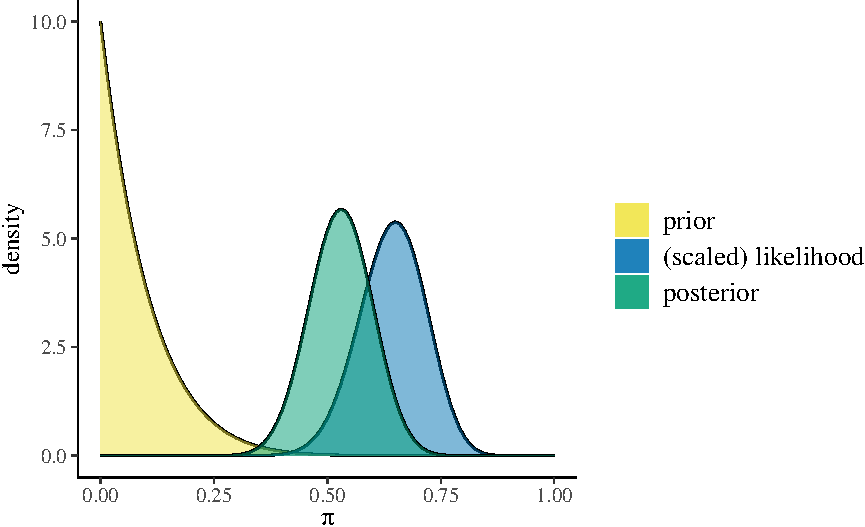
\includegraphics[width=0.8\linewidth]{053_reglin3_files/figure-latex/unnamed-chunk-17-1} \end{center}

Infine, eseguendo la funzione \texttt{launch\_shinystan(fit)} è possibile analizzare oggetti di classe \texttt{stanfit} mediante le funzionalità del pacchetto \texttt{ShinyStan}.

\hypertarget{interpretazione-dei-parametri}{%
\section{Interpretazione dei parametri}\label{interpretazione-dei-parametri}}

Assegnamo ai parametri la seguente interpretazione.

\begin{itemize}
\tightlist
\item
  L'intercetta pari a 25.8 indica il QI medio dei bamini la cui madre ha un QI = 0. Ovviamente questo non ha alcun significato. Vedremo nel modello successivo come trasformare il modello in modo da potere assegnare all'intercetta un'interpretazione sensata.
\item
  La pendenza di 0.61 indica che, all'aumentare di un punto del QI delle madri, il QI medio dei loro bambini aumenta di 0.61 unità. Se consideriamo la gamma di variazione del QI delle madri nel campione, il QI medio dei bambini cambia di 41 punti. Questo indica un sostanziale effetto del QI delle madri sul QI dei loro bambini:
\end{itemize}

\begin{Shaded}
\begin{Highlighting}[]
\NormalTok{(}\FloatTok{138.89} \SpecialCharTok{{-}} \FloatTok{71.04}\NormalTok{) }\SpecialCharTok{*} \FloatTok{0.61}
\CommentTok{\#\textgreater{} [1] 41.4}
\end{Highlighting}
\end{Shaded}

\begin{itemize}
\tightlist
\item
  Il parametro \(\sigma\) fornisce una stima della dispersione delle osservazioni attorno al valore predetto dal modello di regressione, ovvero fornisce una stima della deviazione standard dei residui attorno alla retta di regressione.
\end{itemize}

\hypertarget{centrare-i-predittori}{%
\subsection{Centrare i predittori}\label{centrare-i-predittori}}

Per migliorare l'interpretazione dell'intercetta possiamo ``centrare'' la \(x\), ovvero esprimere la \(x\) nei termini di scarti dalla media: \(x - \bar{x}\). In tali circostanze, la pendenza della retta di regressione resterà immutata, ma l'intercetta corrisponderà a \(\E(y \mid x = \bar{x})\). Per ottenere questo risultato, modifichiamo i dati da passare a Stan:

\begin{Shaded}
\begin{Highlighting}[]
\NormalTok{data2\_list }\OtherTok{\textless{}{-}} \FunctionTok{list}\NormalTok{(}
  \AttributeTok{N =} \FunctionTok{length}\NormalTok{(df}\SpecialCharTok{$}\NormalTok{kid\_score),}
  \AttributeTok{y =}\NormalTok{ df}\SpecialCharTok{$}\NormalTok{kid\_score,}
  \AttributeTok{x =}\NormalTok{ df}\SpecialCharTok{$}\NormalTok{mom\_iq }\SpecialCharTok{{-}} \FunctionTok{mean}\NormalTok{(df}\SpecialCharTok{$}\NormalTok{mom\_iq)}
\NormalTok{)}
\end{Highlighting}
\end{Shaded}

\noindent
Adattiamo il modello:

\begin{Shaded}
\begin{Highlighting}[]
\NormalTok{fit2 }\OtherTok{\textless{}{-}}\NormalTok{ mod}\SpecialCharTok{$}\FunctionTok{sample}\NormalTok{(}
  \AttributeTok{data =}\NormalTok{ data2\_list,}
  \AttributeTok{iter\_sampling =}\NormalTok{ 4000L,}
  \AttributeTok{iter\_warmup =}\NormalTok{ 2000L,}
  \AttributeTok{seed =}\NormalTok{ SEED,}
  \AttributeTok{chains =}\NormalTok{ 4L,}
  \AttributeTok{parallel\_chains =}\NormalTok{ 2L,}
  \AttributeTok{refresh =} \DecValTok{0}\NormalTok{,}
  \AttributeTok{thin =} \DecValTok{1}
\NormalTok{)}
\end{Highlighting}
\end{Shaded}

\noindent
Trasformiamo l'oggetto \texttt{fit} in un oggetto di classe \texttt{stanfit}:

\begin{Shaded}
\begin{Highlighting}[]
\NormalTok{stanfit }\OtherTok{\textless{}{-}}\NormalTok{ rstan}\SpecialCharTok{::}\FunctionTok{read\_stan\_csv}\NormalTok{(fit2}\SpecialCharTok{$}\FunctionTok{output\_files}\NormalTok{())}
\end{Highlighting}
\end{Shaded}

\noindent
Le stime a posteriori dei parametri si ottengono con

\begin{Shaded}
\begin{Highlighting}[]
\NormalTok{fit2}\SpecialCharTok{$}\FunctionTok{summary}\NormalTok{(}\FunctionTok{c}\NormalTok{(}\StringTok{"alpha"}\NormalTok{, }\StringTok{"beta"}\NormalTok{, }\StringTok{"sigma"}\NormalTok{))}
\CommentTok{\#\textgreater{} \# A tibble: 3 x 10}
\CommentTok{\#\textgreater{}   variable   mean median     sd    mad     q5    q95  rhat ess\_bulk ess\_tail}
\CommentTok{\#\textgreater{}   \textless{}chr\textgreater{}     \textless{}dbl\textgreater{}  \textless{}dbl\textgreater{}  \textless{}dbl\textgreater{}  \textless{}dbl\textgreater{}  \textless{}dbl\textgreater{}  \textless{}dbl\textgreater{} \textless{}dbl\textgreater{}    \textless{}dbl\textgreater{}    \textless{}dbl\textgreater{}}
\CommentTok{\#\textgreater{} 1 alpha    86.8   86.8   0.872  0.863  85.4   88.2    1.00   16613.   12276.}
\CommentTok{\#\textgreater{} 2 beta      0.610  0.609 0.0591 0.0592  0.512  0.708  1.00   17947.   12419.}
\CommentTok{\#\textgreater{} 3 sigma    18.3   18.3   0.616  0.616  17.3   19.3    1.00   16622.   11073.}
\end{Highlighting}
\end{Shaded}

\noindent
Si noti che la nuova intercetta, ovvero 86.8, corrisponde al QI medio dei bambini le cui madri hanno un QI pari alla media del campione. Centrare i dati consente dunque di assegnare un'interpretazione utile all'intercetta.

\hypertarget{inference-reg-lin-stan}{%
\chapter{Inferenza sul modello di regressione}\label{inference-reg-lin-stan}}

I minimi quadrati o la massima verosimiglianza trovano i parametri che meglio si adattano ai dati (secondo un criterio prestabilito), ma senza altrimenti vincolare la stima. Ma di solito il ricercatore dispone di informazioni preliminari sui parametri del modello. L'inferenza bayesiana produce invece un compromesso tra tali informazioni pregresse e i dati.

La soluzione dei minimi quadrati è una stima puntuale che rappresenta il vettore dei coefficienti che fornisce il miglior adattamento complessivo ai dati. Per un modello bayesiano, la stima puntuale corrispondente è la \emph{moda a posteriori}, che fornisce il miglior adattamento complessivo ai dati e alla distribuzione a priori. Si noti inoltre che la stima dei minimi quadrati (o di massima verosimiglianza) corrisponde alla moda a posteriori di un modello bayesiano con una distribuzione a priori uniforme.

\hypertarget{rappresentazione-grafica-dellincertezza-della-stima}{%
\section{Rappresentazione grafica dell'incertezza della stima}\label{rappresentazione-grafica-dellincertezza-della-stima}}

Un primo modo per rappresentare l'incertezza dell'inferenza in un ottica bayesiana è quella di rappresentare graficamente la retta di regressione. Continuando con l'esempio descritto nel Capitolo precedente (ovvero, i dati \texttt{kid\_score} e \texttt{mom\_iq} centrati), usando la funzione \texttt{extract()}, salvo le stime a posteriori dei parametri in formato \texttt{list}:

\begin{Shaded}
\begin{Highlighting}[]
\NormalTok{stanfit }\OtherTok{\textless{}{-}}\NormalTok{ rstan}\SpecialCharTok{::}\FunctionTok{read\_stan\_csv}\NormalTok{(fit2}\SpecialCharTok{$}\FunctionTok{output\_files}\NormalTok{())}
\NormalTok{posterior }\OtherTok{\textless{}{-}} \FunctionTok{extract}\NormalTok{(stanfit)}
\end{Highlighting}
\end{Shaded}

Un diagramma a dispersione dei dati con sovrapposto il valore atteso della \(y\) in base al modello bayesiano si ottiene nel modo seguente:

\begin{Shaded}
\begin{Highlighting}[]
\FunctionTok{plot}\NormalTok{(}
\NormalTok{  df}\SpecialCharTok{$}\NormalTok{kid\_score }\SpecialCharTok{\textasciitilde{}} \FunctionTok{I}\NormalTok{(df}\SpecialCharTok{$}\NormalTok{mom\_iq }\SpecialCharTok{{-}} \FunctionTok{mean}\NormalTok{(df}\SpecialCharTok{$}\NormalTok{mom\_iq)), }
  \AttributeTok{pch =} \DecValTok{20}\NormalTok{,}
  \AttributeTok{xlab =} \StringTok{"mom\_iq (centered)"}\NormalTok{,}
  \AttributeTok{ylab =} \StringTok{"kid\_score"}
\NormalTok{)}
\FunctionTok{abline}\NormalTok{(}\FunctionTok{mean}\NormalTok{(posterior}\SpecialCharTok{$}\NormalTok{alpha), }\FunctionTok{mean}\NormalTok{(posterior}\SpecialCharTok{$}\NormalTok{beta), }\AttributeTok{col =} \DecValTok{6}\NormalTok{, }\AttributeTok{lw =} \DecValTok{2}\NormalTok{)}
\end{Highlighting}
\end{Shaded}

\begin{center}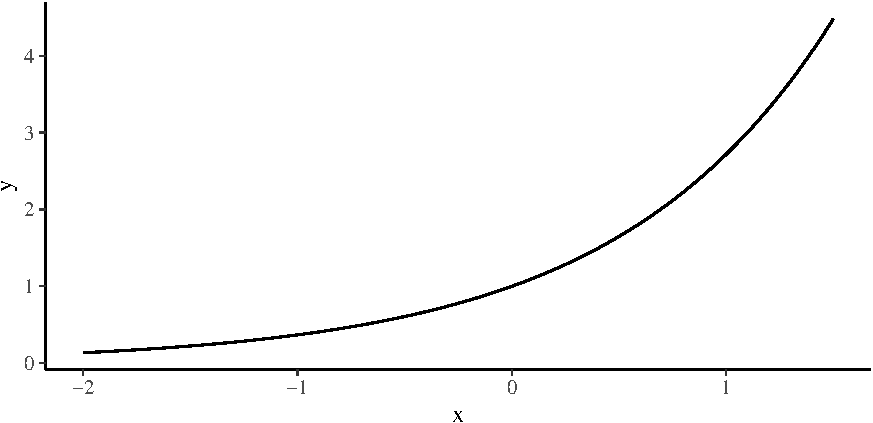
\includegraphics[width=0.8\linewidth]{054_reglin4_files/figure-latex/unnamed-chunk-4-1} \end{center}

Un modo per visualizzare l'incertezza della stima della retta di regressione è quello di tracciare molteplici rette di regressione, ciascuna delle quali definita da una diversa stima dei parametri \(\alpha\) e \(\beta\) che vengono estratti a caso dalle rispettive distribuzioni a posteriori.

\begin{Shaded}
\begin{Highlighting}[]
\FunctionTok{plot}\NormalTok{(}
\NormalTok{  df}\SpecialCharTok{$}\NormalTok{kid\_score }\SpecialCharTok{\textasciitilde{}} \FunctionTok{I}\NormalTok{(df}\SpecialCharTok{$}\NormalTok{mom\_iq }\SpecialCharTok{{-}} \FunctionTok{mean}\NormalTok{(df}\SpecialCharTok{$}\NormalTok{mom\_iq)), }
  \AttributeTok{pch =} \DecValTok{20}\NormalTok{,}
  \AttributeTok{xlab =} \StringTok{"mom\_iq (centered)"}\NormalTok{,}
  \AttributeTok{ylab =} \StringTok{"kid\_score"}
\NormalTok{)}
\ControlFlowTok{for}\NormalTok{ (i }\ControlFlowTok{in} \DecValTok{1}\SpecialCharTok{:}\DecValTok{50}\NormalTok{) \{}
 \FunctionTok{abline}\NormalTok{(posterior}\SpecialCharTok{$}\NormalTok{alpha[i], posterior}\SpecialCharTok{$}\NormalTok{beta[i], }\AttributeTok{col =} \StringTok{"gray"}\NormalTok{, }\AttributeTok{lty =} \DecValTok{1}\NormalTok{)}
\NormalTok{\}}
\FunctionTok{abline}\NormalTok{(}\FunctionTok{mean}\NormalTok{(posterior}\SpecialCharTok{$}\NormalTok{alpha), }\FunctionTok{mean}\NormalTok{(posterior}\SpecialCharTok{$}\NormalTok{beta), }\AttributeTok{col =} \DecValTok{6}\NormalTok{, }\AttributeTok{lw =} \DecValTok{2}\NormalTok{)}
\end{Highlighting}
\end{Shaded}

\begin{center}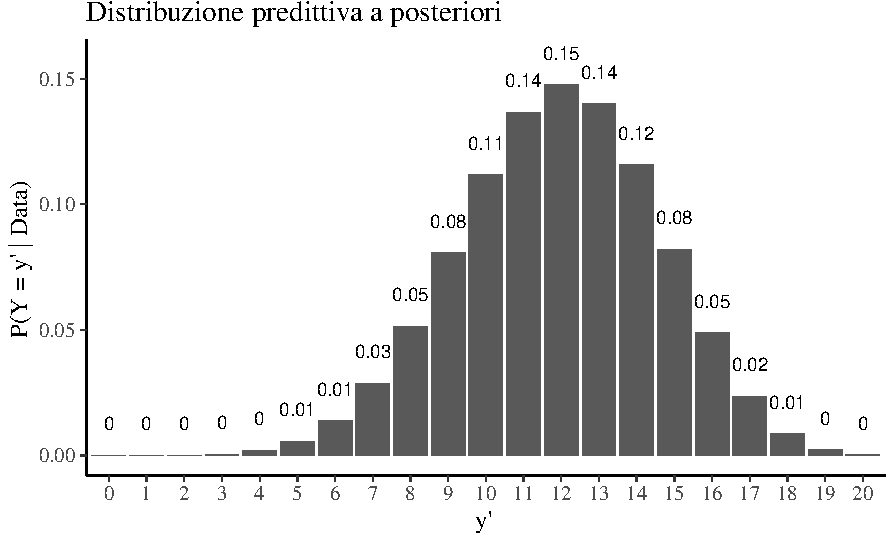
\includegraphics[width=0.8\linewidth]{054_reglin4_files/figure-latex/unnamed-chunk-5-1} \end{center}

\hypertarget{intervalli-di-credibilituxe0}{%
\section{Intervalli di credibilità}\label{intervalli-di-credibilituxe0}}

L'incertezza inferenziale sui parametri può anche essere rappresentata mediante gli \emph{intervalli di credibilità}, ovvero gli intervalli che contengono la quota desiderata (es., il 95\%) della distribuzione a posteriori.

Per l'esempio che stiamo discutendo, gli intervalli di credibilità al 95\% si ottengono nel modo seguente:

\begin{Shaded}
\begin{Highlighting}[]
\NormalTok{posterior }\OtherTok{\textless{}{-}} \FunctionTok{extract}\NormalTok{(stanfit)}
\NormalTok{rstantools}\SpecialCharTok{::}\FunctionTok{posterior\_interval}\NormalTok{(}\FunctionTok{as.matrix}\NormalTok{(stanfit), }\AttributeTok{prob =} \FloatTok{0.95}\NormalTok{)}
\CommentTok{\#\textgreater{}                2.5\%     97.5\%}
\CommentTok{\#\textgreater{} alpha\_std   {-}0.0838    0.0845}
\CommentTok{\#\textgreater{} beta\_std     0.3633    0.5324}
\CommentTok{\#\textgreater{} sigma\_std    0.8404    0.9580}
\CommentTok{\#\textgreater{} alpha       85.0865   88.5229}
\CommentTok{\#\textgreater{} beta         0.4943    0.7244}
\CommentTok{\#\textgreater{} sigma       17.1538   19.5538}
\CommentTok{\#\textgreater{} lp\_\_      {-}172.8280 {-}168.2490}
\end{Highlighting}
\end{Shaded}

Un grafico che riporta l'intervallo di credibilità ai livelli di probabilità desiderati per \(\beta\) si ottiene con le seguenti istruzioni:

\begin{Shaded}
\begin{Highlighting}[]
\FunctionTok{mcmc\_areas}\NormalTok{(}
\NormalTok{  fit2}\SpecialCharTok{$}\FunctionTok{draws}\NormalTok{(}\FunctionTok{c}\NormalTok{(}\StringTok{"beta"}\NormalTok{)),}
  \AttributeTok{prob =} \FloatTok{0.8}\NormalTok{,}
  \AttributeTok{prob\_outer =} \FloatTok{0.95}
\NormalTok{  )}
\end{Highlighting}
\end{Shaded}

\begin{center}\includegraphics[width=0.8\linewidth]{054_reglin4_files/figure-latex/unnamed-chunk-7-1} \end{center}

Per i parametri ottenuti analizzando i dati standardizzati, abbiamo

\begin{Shaded}
\begin{Highlighting}[]
\NormalTok{stanfit }\SpecialCharTok{\%\textgreater{}\%}
  \FunctionTok{mcmc\_intervals}\NormalTok{(}
    \AttributeTok{pars =} \FunctionTok{c}\NormalTok{(}\StringTok{"alpha\_std"}\NormalTok{, }\StringTok{"beta\_std"}\NormalTok{, }\StringTok{"sigma\_std"}\NormalTok{), }
    \AttributeTok{prob =} \FloatTok{0.8}\NormalTok{,}
    \AttributeTok{prob\_outer =} \FloatTok{0.95}
\NormalTok{  )}
\end{Highlighting}
\end{Shaded}

\begin{center}\includegraphics[width=0.8\linewidth]{054_reglin4_files/figure-latex/unnamed-chunk-8-1} \end{center}

\hypertarget{rappresentazione-grafica-della-distribuzione-a-posteriori}{%
\section{Rappresentazione grafica della distribuzione a posteriori}\label{rappresentazione-grafica-della-distribuzione-a-posteriori}}

Non c'è niente di ``magico'' o necessario relativamente al livello di 0.95: il valore 0.95 è arbitrario. Sono possibili tantissime altre soglie per quantificare la nostra incertezza: alcuni ricercatori usano il livello di 0.89, altri quello di 0.5. Se l'obiettivo è quello di descrivere il livello della nostra incertezza relativamente alla stima del parametro, allora dobbiamo riconoscere che la nostra incertezza è descritta dall'\emph{intera} distribuzione a posteriori. Per cui il metodo più semplice, più diretto e più completo per descrivere la nostra incertezza rispetto alla stima dei parametri è quello di riportare graficamente tutta la distribuzione a posteriori. Una rappresentazione della distribuzione a posteriori dei parametri del modello dell'esempio si ottiene nel modo seguente:

\begin{Shaded}
\begin{Highlighting}[]
\FunctionTok{stan\_dens}\NormalTok{(}
\NormalTok{  stanfit, }
  \AttributeTok{pars =} \FunctionTok{c}\NormalTok{(}\StringTok{"alpha"}\NormalTok{, }\StringTok{"beta"}\NormalTok{, }\StringTok{"sigma"}\NormalTok{),}
  \AttributeTok{fill =} \StringTok{"\#4ca5ff"}
\NormalTok{)}
\end{Highlighting}
\end{Shaded}

\begin{center}\includegraphics[width=0.8\linewidth]{054_reglin4_files/figure-latex/unnamed-chunk-9-1} \end{center}

\hypertarget{test-di-ipotesi}{%
\section{Test di ipotesi}\label{test-di-ipotesi}}

In Stan è facile valutare ipotesi direzionali. Per esempio, la probabilità di \(\hat{\beta} > 0\) è

\begin{Shaded}
\begin{Highlighting}[]
\FunctionTok{sum}\NormalTok{(posterior}\SpecialCharTok{$}\NormalTok{beta }\SpecialCharTok{\textgreater{}} \DecValTok{0}\NormalTok{) }\SpecialCharTok{/} \FunctionTok{length}\NormalTok{(posterior}\SpecialCharTok{$}\NormalTok{beta)}
\CommentTok{\#\textgreater{} [1] 1}
\end{Highlighting}
\end{Shaded}

\hypertarget{regressione-robusta}{%
\section{Regressione robusta}\label{regressione-robusta}}

Spesso i ricercatori devono affrontare il problema degli outlier: in presenza di outlier, un modello statistico basato sulla distribuzione Normale produrrà delle stime dei parametri che non si generalizzano ad altri campioni di dati. Il metodo tradizoinale per affrontare questo problema è quello di eliminare gli outlier prima di eseguire l'analisi statistica. Il problema di questo approccio, però, è che il criterio utilizzato per eliminare gli outlier, quale esso sia, è arbitrario; dunque, usando criteri diversi per eliminare gli outlier, i ricercatori finiscono per trovare risultati diversi.

Questo problema trova una semplice soluzione nell'approccio bayesiano. Nel modello di regressione che abbiamo dicusso finora è stato ipotizzato che \(\varepsilon \sim \mathcal{N}(0, \sigma_{\varepsilon})\). Per un modello formulato in questi termini, la presenza di solo un valore anomalo e influente può avere un effetto drammatico sulle stime dei parametri.

Per fare un esempio, introduciamo un singlo valore anomalo nel set dei dati dell'esempio che stiamo discutendo:

\begin{Shaded}
\begin{Highlighting}[]
\NormalTok{df2 }\OtherTok{\textless{}{-}}\NormalTok{ df}
\NormalTok{df2}\SpecialCharTok{$}\NormalTok{kid\_score[}\DecValTok{434}\NormalTok{] }\OtherTok{\textless{}{-}} \SpecialCharTok{{-}}\DecValTok{500}
\NormalTok{df2}\SpecialCharTok{$}\NormalTok{mom\_iq[}\DecValTok{434}\NormalTok{] }\OtherTok{\textless{}{-}} \DecValTok{140}
\end{Highlighting}
\end{Shaded}

Per comodità, calcoliamo le stime di \(\alpha\) e \(\beta\) con il metodo dei minimi quadrati (le stime dei parametri sono simili a quelle di un modello bayesiano Normale con distribuzioni a priori vagamente informative). Sappiamo che, nel campione originari di dati, \(\hat{\beta} \approx 0.6\). In presenza di un solo outlier troviamo
che

\begin{Shaded}
\begin{Highlighting}[]
\FunctionTok{coef}\NormalTok{(}\FunctionTok{lm}\NormalTok{(kid\_score }\SpecialCharTok{\textasciitilde{}}\NormalTok{ mom\_iq, }\AttributeTok{data =}\NormalTok{ df2))}
\CommentTok{\#\textgreater{} (Intercept)      mom\_iq }
\CommentTok{\#\textgreater{}      49.188       0.363}
\end{Highlighting}
\end{Shaded}

\noindent
la stima di \(\beta\) viene drammaticamente ridotta (di quasi la metà!).

Non è però necessario assumere \(\varepsilon \sim \mathcal{N}(0, \sigma_{\varepsilon})\). È altrettanto valido un modello che ipotizza una diversa distribuzione di densità per i residui come, ad esempio, la distribuzione \(t\) di Student con un piccolo numero di gradi di libertà. Una caratteristica della \(t\) di Student è che le code della distribuzione contengono una massa di probabilità maggiore della Normale. Ciò fornisce alla \(t\) di Student la possibilità di ``rendere conto'' della presenza di osservazioni lontane dalla media della distribuzione. In altri termini, se in modello di regressione usiamo la \(t\) di Student quale distribuzione dei residui, la presenza di outlier avrà una minore influenza sulle stime dei parametri di quanto avvenga nel modello Normale.

Per verificare questa affermazione, modifichiamo il codice Stan in modo tale da ipotizzare che la distribuzione della \(y\) segua una \(t\) di Student con un numero \(\nu\) gradi di libertà stimato dal modello: \texttt{student\_t(nu,\ mu,\ sigma)}.\footnote{È equivalente scrivere
  \[
  y_i = \mu_i + \varepsilon_i, \quad \text{dove } \mu_i = \alpha + \beta x_i, \varepsilon_i \sim \mathcal{N}(0, \sigma_\varepsilon),
  \]
  oppure
  \[
  y_i \sim \mathcal{N}(\mu_i, \sigma_\varepsilon).
  \]}

\begin{Shaded}
\begin{Highlighting}[]
\NormalTok{modelString }\OtherTok{=} \StringTok{"}
\StringTok{data \{}
\StringTok{  int\textless{}lower=0\textgreater{} N;}
\StringTok{  vector[N] y;}
\StringTok{  vector[N] x;}
\StringTok{\}}
\StringTok{transformed data \{}
\StringTok{  vector[N] x\_std;}
\StringTok{  vector[N] y\_std;}
\StringTok{  x\_std = (x {-} mean(x)) / sd(x);}
\StringTok{  y\_std = (y {-} mean(y)) / sd(y);}
\StringTok{\}}
\StringTok{parameters \{}
\StringTok{  real alpha\_std;}
\StringTok{  real beta\_std;}
\StringTok{  real\textless{}lower=0\textgreater{} sigma\_std;}
\StringTok{  real\textless{}lower=1\textgreater{} nu;    // degrees of freedom is constrained \textgreater{}1}
\StringTok{\}}
\StringTok{model \{}
\StringTok{  alpha\_std \textasciitilde{} normal(0, 2);}
\StringTok{  beta\_std \textasciitilde{} normal(0, 2);}
\StringTok{  sigma\_std \textasciitilde{} cauchy(0, 2);}
\StringTok{  nu \textasciitilde{} gamma(2, 0.1);   // Juárez and Steel(2010)}
\StringTok{  y\_std \textasciitilde{} student\_t(nu, alpha\_std + beta\_std * x\_std, sigma\_std);}
\StringTok{\}}
\StringTok{generated quantities \{}
\StringTok{  real alpha;}
\StringTok{  real beta;}
\StringTok{  real\textless{}lower=0\textgreater{} sigma;}
\StringTok{  alpha = sd(y) * (alpha\_std {-} beta\_std * mean(x) / sd(x))}
\StringTok{           + mean(y);}
\StringTok{  beta = beta\_std * sd(y) / sd(x);}
\StringTok{  sigma = sd(y) * sigma\_std;}
\StringTok{\}}
\StringTok{"}
\FunctionTok{writeLines}\NormalTok{(modelString, }\AttributeTok{con =} \StringTok{"code/simpleregstdrobust.stan"}\NormalTok{)}
\end{Highlighting}
\end{Shaded}

\noindent
Costruiamo la lista dei dati usando il data.frame \texttt{df2} che include l'outlier:

\begin{Shaded}
\begin{Highlighting}[]
\NormalTok{data3\_list }\OtherTok{\textless{}{-}} \FunctionTok{list}\NormalTok{(}
  \AttributeTok{N =} \FunctionTok{length}\NormalTok{(df2}\SpecialCharTok{$}\NormalTok{kid\_score),}
  \AttributeTok{y =}\NormalTok{ df2}\SpecialCharTok{$}\NormalTok{kid\_score,}
  \AttributeTok{x =}\NormalTok{ df2}\SpecialCharTok{$}\NormalTok{mom\_iq }\SpecialCharTok{{-}} \FunctionTok{mean}\NormalTok{(df2}\SpecialCharTok{$}\NormalTok{mom\_iq)}
\NormalTok{)}
\end{Highlighting}
\end{Shaded}

\noindent
Adattiamo il modello di regressione robusta ai dati:

\begin{Shaded}
\begin{Highlighting}[]
\NormalTok{file }\OtherTok{\textless{}{-}} \FunctionTok{file.path}\NormalTok{(}\StringTok{"code"}\NormalTok{, }\StringTok{"simpleregstdrobust.stan"}\NormalTok{)}
\NormalTok{mod }\OtherTok{\textless{}{-}} \FunctionTok{cmdstan\_model}\NormalTok{(file)}

\NormalTok{fit4 }\OtherTok{\textless{}{-}}\NormalTok{ mod}\SpecialCharTok{$}\FunctionTok{sample}\NormalTok{(}
  \AttributeTok{data =}\NormalTok{ data3\_list,}
  \AttributeTok{iter\_sampling =}\NormalTok{ 4000L,}
  \AttributeTok{iter\_warmup =}\NormalTok{ 2000L,}
  \AttributeTok{seed =}\NormalTok{ SEED,}
  \AttributeTok{chains =}\NormalTok{ 4L,}
  \AttributeTok{parallel\_chains =}\NormalTok{ 2L,}
  \AttributeTok{refresh =} \DecValTok{0}\NormalTok{,}
  \AttributeTok{thin =} \DecValTok{1}
\NormalTok{)}
\end{Highlighting}
\end{Shaded}

\noindent
Esaminando le stime dei parametri

\begin{Shaded}
\begin{Highlighting}[]
\NormalTok{fit4}\SpecialCharTok{$}\FunctionTok{summary}\NormalTok{(}\FunctionTok{c}\NormalTok{(}\StringTok{"alpha"}\NormalTok{, }\StringTok{"beta"}\NormalTok{, }\StringTok{"sigma"}\NormalTok{, }\StringTok{"nu"}\NormalTok{))}
\CommentTok{\#\textgreater{} \# A tibble: 4 x 10}
\CommentTok{\#\textgreater{}   variable   mean median     sd    mad     q5    q95  rhat ess\_bulk ess\_tail}
\CommentTok{\#\textgreater{}   \textless{}chr\textgreater{}     \textless{}dbl\textgreater{}  \textless{}dbl\textgreater{}  \textless{}dbl\textgreater{}  \textless{}dbl\textgreater{}  \textless{}dbl\textgreater{}  \textless{}dbl\textgreater{} \textless{}dbl\textgreater{}    \textless{}dbl\textgreater{}    \textless{}dbl\textgreater{}}
\CommentTok{\#\textgreater{} 1 alpha    87.8   87.8   0.887  0.899  86.3   89.3    1.00   13776.   11987.}
\CommentTok{\#\textgreater{} 2 beta      0.603  0.603 0.0585 0.0577  0.506  0.698  1.00   14185.   11067.}
\CommentTok{\#\textgreater{} 3 sigma    15.9   15.9   0.806  0.812  14.6   17.3    1.00   12699.   11256.}
\CommentTok{\#\textgreater{} 4 nu        5.58   5.44  1.15   1.11    3.94   7.65   1.00   12258.   12033.}
\end{Highlighting}
\end{Shaded}

\noindent
notiamo che la stima di \(\beta\) è rimasta praticamente immutata. La regressione ``robusta'' non risente dunque della presenza degli outlier.

\hypertarget{comparison-two-means-stan}{%
\chapter{Confronto tra due gruppi indipendenti}\label{comparison-two-means-stan}}

Il problema del confronto tra due gruppi indipendenti può essere formulato nei termini di un modello di regressione nel quale la variabile \(x\) è dicotomica, ovvero assume solo due valori.

\hypertarget{regressione-lineare-con-una-variabile-dicotomica}{%
\section{Regressione lineare con una variabile dicotomica}\label{regressione-lineare-con-una-variabile-dicotomica}}

Se \(x\) è una variabile dicotomica con valori 0 e 1, allora per il modello di regressione \(\mu_i = \alpha + \beta x_i\) abbiamo quanto segue. Quando \(x=0\), il modello diventa
\[
\mu_i = \alpha
\]
\noindent
mentre, quando \(X=1\), il modello diventa
\[
\mu_i = \alpha + \beta.
\]
\noindent
Ciò significa che il parametro \(\alpha\) è uguale al valore atteso del gruppo codificato con \(X=0\) e il parametro \(\beta\) è uguale alla differenza tra le medie dei due gruppi (essendo la media del secondo gruppo uguale a \(\alpha + \beta\)). Il parametro \(\beta\), dunque, codifica l'effetto di una manipolazione sperimentale o di un trattamento, e l'inferenza su \(\beta\) corrisponde direttamente all'inferenza sull'efficacia di un trattamento o di un effetto sperimentale.\footnote{Per ``effetto di un trattamento'' si intende la differenza tra le medie di due gruppi (per esempio, il gruppo ``sperimentale'' e il gruppo ``di controllo'').} L'inferenza su \(\beta\), dunque, viene utilizzata per capire quanto ``credibile'' può essere considerato l'effetto di un trattamento o di una manipolazione sperimentale.

\hypertarget{un-esempio-concreto}{%
\subsection{Un esempio concreto}\label{un-esempio-concreto}}

Esaminiamo nuovamente un sottoinsieme di dati tratto dal \emph{National Longitudinal Survey of Youth} i quali sono stati discussi da \textcite{gelman2020regression}. I soggetti sono bambini di 3 e 4 anni. La variabile dipendente, \texttt{kid\_score}, è il punteggio totale del \emph{Peabody Individual Achievement Test} (PIAT) costituito dalla somma dei punteggi di tre sottoscale (Mathematics, Reading comprehension, Reading recognition). La variabile indipendente, \texttt{mom\_hs}, è il livello di istruzione della madre, codificato con due livelli: scuola media superiore completata oppure no. La domanda della ricerca è se il QI del figlio (misurato sulla scala PIAT) risulta o meno associato al livello di istruzione della madre.

Codifichiamo il livello di istruzione della madre (\(x\)) con una \emph{variabile indicatrice} (ovvero, una variabile che assume solo i valori 0 e 1) tale per cui:

\begin{itemize}
\item
  \(x=0\): la madre non ha completato la scuola secondaria di secondo grado (scuola media superiore);
\item
  \(x=1\): la madre ha completato la scuola media superiore.
\end{itemize}

\noindent
Supponiamo che i dati siano contenuti nel data.frame \texttt{df}.

\begin{Shaded}
\begin{Highlighting}[]
\FunctionTok{library}\NormalTok{(}\StringTok{"foreign"}\NormalTok{)}
\NormalTok{df }\OtherTok{\textless{}{-}} \FunctionTok{read.dta}\NormalTok{(}\FunctionTok{here}\NormalTok{(}\StringTok{"data"}\NormalTok{, }\StringTok{"kidiq.dta"}\NormalTok{))}
\end{Highlighting}
\end{Shaded}

\noindent
Calcoliamo le statistiche descrittive per i due gruppi:

\begin{Shaded}
\begin{Highlighting}[]
\NormalTok{df }\SpecialCharTok{\%\textgreater{}\%} 
  \FunctionTok{group\_by}\NormalTok{(mom\_hs) }\SpecialCharTok{\%\textgreater{}\%} 
  \FunctionTok{summarise}\NormalTok{(}
    \AttributeTok{mean\_kid\_score =} \FunctionTok{mean}\NormalTok{(kid\_score),}
    \AttributeTok{std =} \FunctionTok{sqrt}\NormalTok{(}\FunctionTok{var}\NormalTok{(kid\_score))}
\NormalTok{  )}
\CommentTok{\#\textgreater{} \# A tibble: 2 x 3}
\CommentTok{\#\textgreater{}   mom\_hs mean\_kid\_score   std}
\CommentTok{\#\textgreater{}    \textless{}dbl\textgreater{}          \textless{}dbl\textgreater{} \textless{}dbl\textgreater{}}
\CommentTok{\#\textgreater{} 1      0           77.5  22.6}
\CommentTok{\#\textgreater{} 2      1           89.3  19.0}
\end{Highlighting}
\end{Shaded}

\noindent
Il punteggio medio PIAT è pari a 77.5 per i bambini la cui madre non ha il diploma di scuola media superiore e pari a 89.3 per i bambini la cui madre ha completato la scuola media superiore. Questa differenza suggerisce un'associazione tra le variabili, ma tale differenza potrebbe essere soltanto la conseguenza della variabilità campionaria, senza riflettere una caratteristica generale della popolazione. Come possiamo usare il modello statistico lineare per fare inferenza sulla differenza osservata tra i due gruppi? Non dobbiamo fare nient'altro che usare lo stesso modello di regressione che abbiamo definito in precedenza.

\begin{Shaded}
\begin{Highlighting}[]
\NormalTok{modelString }\OtherTok{=} \StringTok{"}
\StringTok{data \{}
\StringTok{  int\textless{}lower=0\textgreater{} N;}
\StringTok{  vector[N] y;}
\StringTok{  vector[N] x;}
\StringTok{\}}
\StringTok{transformed data \{}
\StringTok{  vector[N] x\_std;}
\StringTok{  vector[N] y\_std;}
\StringTok{  x\_std = (x {-} mean(x)) / sd(x);}
\StringTok{  y\_std = (y {-} mean(y)) / sd(y);}
\StringTok{\}}
\StringTok{parameters \{}
\StringTok{  real alpha\_std;}
\StringTok{  real beta\_std;}
\StringTok{  real\textless{}lower=0\textgreater{} sigma\_std;}
\StringTok{\}}
\StringTok{model \{}
\StringTok{  alpha\_std \textasciitilde{} normal(0, 2);}
\StringTok{  beta\_std \textasciitilde{} normal(0, 2);}
\StringTok{  sigma\_std \textasciitilde{} cauchy(0, 2);}
\StringTok{  y\_std \textasciitilde{} normal(alpha\_std + beta\_std * x\_std, sigma\_std);}
\StringTok{\}}
\StringTok{generated quantities \{}
\StringTok{  real alpha;}
\StringTok{  real beta;}
\StringTok{  real\textless{}lower=0\textgreater{} sigma;}
\StringTok{  alpha = sd(y) * (alpha\_std {-} beta\_std * mean(x) / sd(x))}
\StringTok{           + mean(y);}
\StringTok{  beta = beta\_std * sd(y) / sd(x);}
\StringTok{  sigma = sd(y) * sigma\_std;}
\StringTok{\}}
\StringTok{"}
\FunctionTok{writeLines}\NormalTok{(modelString, }\AttributeTok{con =} \StringTok{"code/simpleregstd.stan"}\NormalTok{)}
\end{Highlighting}
\end{Shaded}

\noindent
Come in precedenza, salviamo i dati in un oggetto di classe \texttt{list}:

\begin{Shaded}
\begin{Highlighting}[]
\NormalTok{data\_list }\OtherTok{\textless{}{-}} \FunctionTok{list}\NormalTok{(}
  \AttributeTok{N =} \FunctionTok{length}\NormalTok{(df}\SpecialCharTok{$}\NormalTok{kid\_score),}
  \AttributeTok{y =}\NormalTok{ df}\SpecialCharTok{$}\NormalTok{kid\_score,}
  \AttributeTok{x =}\NormalTok{ df}\SpecialCharTok{$}\NormalTok{mom\_hs}
\NormalTok{)}
\end{Highlighting}
\end{Shaded}

\noindent
Compiliamo il modello:

\begin{Shaded}
\begin{Highlighting}[]
\NormalTok{file }\OtherTok{\textless{}{-}} \FunctionTok{file.path}\NormalTok{(}\StringTok{"code"}\NormalTok{, }\StringTok{"simpleregstd.stan"}\NormalTok{)}
\NormalTok{mod }\OtherTok{\textless{}{-}} \FunctionTok{cmdstan\_model}\NormalTok{(file)}
\end{Highlighting}
\end{Shaded}

\noindent
Adattiamo il modello ai dati:

\begin{Shaded}
\begin{Highlighting}[]
\NormalTok{fit }\OtherTok{\textless{}{-}}\NormalTok{ mod}\SpecialCharTok{$}\FunctionTok{sample}\NormalTok{(}
  \AttributeTok{data =}\NormalTok{ data\_list,}
  \AttributeTok{iter\_sampling =}\NormalTok{ 4000L,}
  \AttributeTok{iter\_warmup =}\NormalTok{ 2000L,}
  \AttributeTok{seed =}\NormalTok{ SEED,}
  \AttributeTok{chains =}\NormalTok{ 4L,}
  \AttributeTok{parallel\_chains =}\NormalTok{ 2L,}
  \AttributeTok{refresh =} \DecValTok{0}\NormalTok{,}
  \AttributeTok{thin =} \DecValTok{1}
\NormalTok{)}
\end{Highlighting}
\end{Shaded}

\begin{Shaded}
\begin{Highlighting}[]
\NormalTok{stanfit }\OtherTok{\textless{}{-}}\NormalTok{ rstan}\SpecialCharTok{::}\FunctionTok{read\_stan\_csv}\NormalTok{(fit}\SpecialCharTok{$}\FunctionTok{output\_files}\NormalTok{())}
\NormalTok{posterior }\OtherTok{\textless{}{-}} \FunctionTok{extract}\NormalTok{(stanfit)}
\end{Highlighting}
\end{Shaded}

\begin{Shaded}
\begin{Highlighting}[]
\FunctionTok{plot}\NormalTok{(}
\NormalTok{  df}\SpecialCharTok{$}\NormalTok{kid\_score }\SpecialCharTok{\textasciitilde{}}\NormalTok{ df}\SpecialCharTok{$}\NormalTok{mom\_hs, }
  \AttributeTok{pch =} \DecValTok{20}\NormalTok{,}
  \AttributeTok{xlab =} \StringTok{"mom\_hs"}\NormalTok{,}
  \AttributeTok{ylab =} \StringTok{"kid\_score"}
\NormalTok{)}
\FunctionTok{abline}\NormalTok{(}\FunctionTok{mean}\NormalTok{(posterior}\SpecialCharTok{$}\NormalTok{alpha), }\FunctionTok{mean}\NormalTok{(posterior}\SpecialCharTok{$}\NormalTok{beta), }\AttributeTok{col =} \DecValTok{6}\NormalTok{, }\AttributeTok{lw =} \DecValTok{2}\NormalTok{)}
\end{Highlighting}
\end{Shaded}

\begin{center}\includegraphics[width=0.8\linewidth]{055_reglin5_files/figure-latex/unnamed-chunk-9-1} \end{center}

\noindent
Le stime a posteriori dei parametri si ottengono con:

\begin{Shaded}
\begin{Highlighting}[]
\NormalTok{fit}\SpecialCharTok{$}\FunctionTok{summary}\NormalTok{(}\FunctionTok{c}\NormalTok{(}\StringTok{"alpha"}\NormalTok{, }\StringTok{"beta"}\NormalTok{, }\StringTok{"sigma"}\NormalTok{))}
\CommentTok{\#\textgreater{} \# A tibble: 3 x 10}
\CommentTok{\#\textgreater{}   variable  mean median    sd   mad    q5   q95  rhat ess\_bulk ess\_tail}
\CommentTok{\#\textgreater{}   \textless{}chr\textgreater{}    \textless{}dbl\textgreater{}  \textless{}dbl\textgreater{} \textless{}dbl\textgreater{} \textless{}dbl\textgreater{} \textless{}dbl\textgreater{} \textless{}dbl\textgreater{} \textless{}dbl\textgreater{}    \textless{}dbl\textgreater{}    \textless{}dbl\textgreater{}}
\CommentTok{\#\textgreater{} 1 alpha     77.5   77.6 2.07  2.06  74.2   81.0  1.00   17948.   11861.}
\CommentTok{\#\textgreater{} 2 beta      11.8   11.8 2.34  2.33   7.91  15.6  1.00   18036.   12038.}
\CommentTok{\#\textgreater{} 3 sigma     19.9   19.9 0.679 0.673 18.8   21.0  1.00   18897.   11950.}
\end{Highlighting}
\end{Shaded}

I risultati confermano ciò che ci aspettavamo:

\begin{itemize}
\tightlist
\item
  il coefficiente \(\texttt{alpha} = 77.56\) corrisponde alla media del gruppo codificato con \(x = 0\), ovvero la media dei punteggi PIAT per i bambini la cui madre non ha completato la scuola media superiore;
\item
  il coefficiente \(\texttt{beta} = 11.76\) corrisponde alla differenza tra le medie dei due gruppi, ovvero 89.32 - 77.55 = 11.77 (con piccoli errori di approssimazione).
\end{itemize}

La seguente chiamata ritorna l'intervallo di credibilità al 95\% per tutti i parametri del modello:

\begin{Shaded}
\begin{Highlighting}[]
\NormalTok{rstantools}\SpecialCharTok{::}\FunctionTok{posterior\_interval}\NormalTok{(}\FunctionTok{as.matrix}\NormalTok{(stanfit), }\AttributeTok{prob =} \FloatTok{0.95}\NormalTok{)}
\CommentTok{\#\textgreater{}                2.5\%     97.5\%}
\CommentTok{\#\textgreater{} alpha\_std   {-}0.0904    0.0916}
\CommentTok{\#\textgreater{} beta\_std     0.1447    0.3289}
\CommentTok{\#\textgreater{} sigma\_std    0.9120    1.0437}
\CommentTok{\#\textgreater{} alpha       73.4854   81.6092}
\CommentTok{\#\textgreater{} beta         7.1877   16.3437}
\CommentTok{\#\textgreater{} sigma       18.6155   21.3025}
\CommentTok{\#\textgreater{} lp\_\_      {-}209.0430 {-}204.3220}
\end{Highlighting}
\end{Shaded}

Possiamo dunque concludere che i bambini la cui madre ha completato la scuola superiore ottengono in media circa 12 punti in più rispetto ai bambini la cui madre non ha completato la scuola superiore. L'intervallo di credibilità al 95\% ci dice che possiamo essere sicuri al 95\% che tale differenza sia di almeno 7 punti e possa arrivare fino a ben 16 punti. Per riassumere, possiamo concludere, con un grado di certezza soggettiva del 95\%, che c'è un'associazione positiva tra il livello di scolarità della madre e l'intelligenza del bambino: le madri che hanno livello di istruzione più alto della media tendo ad avere bambini il cui QI è anch'esso più alto della media.

\hypertarget{la-dimensione-delleffetto}{%
\section{La dimensione dell'effetto}\label{la-dimensione-delleffetto}}

Avendo a disposizione le informazioni sulle distribuzioni a posteriori dei parametri è facile calcolare la dimensione dell'effetto nei termini del \(d\) di Cohen:

\begin{Shaded}
\begin{Highlighting}[]
\FloatTok{11.75398} \SpecialCharTok{/} \FloatTok{19.90159} 
\CommentTok{\#\textgreater{} [1] 0.591}
\end{Highlighting}
\end{Shaded}

\noindent
Il \(d\) di Cohen di entità ``media'' {[}\(d\) \textgreater{} 0.5; \textcite{sawilowsky2009new}{]} conferma l'importanza dell'influenza della scolarità delle madri sul QI dei bambini.


% Bibliography
%%%%%%%%%%%%%%%%%%%%%%%%%%%%%%%%%%%%%%%%%%%%%%%%%%%%%%%%%%

\backmatter
\SmallMargins

\printbibliography
\onecolumn


% Tables (of tables, of figures)
%%%%%%%%%%%%%%%%%%%%%%%%%%%%%%%%%%%%%%%%%%%%%%%%%%%%%%%%%%


\cleardoublepage
\LargeMargins
\listoffigures


% After-body (LaTeX code inclusion)
%%%%%%%%%%%%%%%%%%%%%%%%%%%%%%%%%%%%%%%%%%%%%%%%%%%%%%%%%%




% Back cover
%%%%%%%%%%%%%%%%%%%%%%%%%%%%%%%%%%%%%%%%%%%%%%%%%%%%%%%%%%%

% Even page, small margins, no running head, no page number.
\evenpage
\SmallMargins
\thispagestyle{empty}

\begin{normalsize}

\begin{description}

\selectlanguage{italian}
\item[Abstract]
This document contains the material of the lessons of Psicometria B000286 (2021/2022) aimed at students of the first year of the Degree Course in Psychological Sciences and Techniques of the University of Florence, Italy.
\item[Keywords]
Data science, Bayesian statistics.
~\\

\end{description}

\end{normalsize}


\end{document}
